%% 
%% Copyright 2007-2025 Elsevier Ltd
%% 
%% This file is part of the 'Elsarticle Bundle'.
%% ---------------------------------------------
%% 
%% It may be distributed under the conditions of the LaTeX Project Public
%% License, either version 1.3 of this license or (at your option) any
%% later version.  The latest version of this license is in
%%    http://www.latex-project.org/lppl.txt
%% and version 1.3 or later is part of all distributions of LaTeX
%% version 1999/12/01 or later.
%% 
%% The list of all files belonging to the 'Elsarticle Bundle' is
%% given in the file `manifest.txt'.
%% 
%% Template article for Elsevier's document class `elsarticle'
%% with harvard style bibliographic references

\documentclass[preprint,12pt,authoryear]{elsarticle}

%% Use the option review to obtain double line spacing
%% \documentclass[authoryear,preprint,review,12pt]{elsarticle}

%% Use the options 1p,twocolumn; 3p; 3p,twocolumn; 5p; or 5p,twocolumn
%% for a journal layout:
%% \documentclass[final,1p,times,authoryear]{elsarticle}
%% \documentclass[final,1p,times,twocolumn,authoryear]{elsarticle}
%% \documentclass[final,3p,times,authoryear]{elsarticle}
%% \documentclass[final,3p,times,twocolumn,authoryear]{elsarticle}
%% \documentclass[final,5p,times,authoryear]{elsarticle}
%% \documentclass[final,5p,times,twocolumn,authoryear]{elsarticle}

%% For including figures, graphicx.sty has been loaded in
%% elsarticle.cls. If you prefer to use the old commands
%% please give \usepackage{epsfig}

%% The amssymb package provides various useful mathematical symbols
\usepackage{amssymb}
%% The amsmath package provides various useful equation environments.
\usepackage{amsmath}
\usepackage{xcolor} 
\usepackage{soul}
\usepackage{booktabs}
\usepackage{tabularx}
\usepackage{float}
\usepackage{subcaption}

%% The amsthm package provides extended theorem environments
%% \usepackage{amsthm}

%% The lineno packages adds line numbers. Start line numbering with
%% \begin{linenumbers}, end it with \end{linenumbers}. Or switch it on
%% for the whole article with \linenumbers.
%% \usepackage{lineno}

%%%%%%%%%%%%%%%%%%%%%%%%%%%%%%%%%%%%%%%%%
\usepackage{amssymb}
\usepackage{ifthen}
\usepackage{xcolor}

\newboolean{showcomments}
\setboolean{showcomments}{true}

\newcommand{\awesomeModel}{PhyEnv-NN }

\ifthenelse{\boolean{showcomments}}
  {
   \newcommand{\nb}[3]{
        {\color{#1}\fbox{\bfseries\sffamily\scriptsize#2}
            {\sf\small$\blacktriangleright$\textit{#3}$\blacktriangleleft$}
        }
   }  
   \newcommand\intupdate[1]{{\color{blue}{#1}}}
   \newcommand\update[1]{\texorpdfstring{\intupdate{#1}}{#1}}
   
   \newcommand\intremove[1]{{{\color{red}{\sout{#1}}}}}
   \newcommand\remove[1]{\texorpdfstring{\intremove{#1}}{#1}}
  }
  {
   \newcommand{\nb}[3]{}
   \newcommand\update[1]{{#1}}
   \newcommand\remove[1]{}
  }

\newcommand\RICCARDO[1]{\nb{orange}{RICCARDO}{#1}}
\newcommand\SIMONE[1]{\nb{teal}{SIMONE}{#1}}
%%%%%%%%%%%%%%%%%%%%%%%%%%%%%%%%%%%%%%%%%

\journal{Ecological Informatics}

\begin{document}

\begin{frontmatter}

%% Title, authors and addresses

%% use the tnoteref command within \title for footnotes;
%% use the tnotetext command for theassociated footnote;
%% use the fnref command within \author or \affiliation for footnotes;
%% use the fntext command for theassociated footnote;
%% use the corref command within \author for corresponding author footnotes;
%% use the cortext command for theassociated footnote;
%% use the ead command for the email address,
%% and the form \ead[url] for the home page:
%% \title{Title\tnoteref{label1}}
%% \tnotetext[label1]{}
%% \author{Name\corref{cor1}\fnref{label2}}
%% \ead{email address}
%% \ead[url]{home page}
%% \fntext[label2]{}
%% \cortext[cor1]{}
%% \affiliation{organization={},
%%            addressline={}, 
%%            city={},
%%            postcode={}, 
%%            state={},
%%            country={}}
%% \fntext[label3]{}

\title{Where does information about plant trait variation reside? A predictive analysis of phylogenetic and environmental information in New Zealand ferns}

%% use optional labels to link authors explicitly to addresses:
%% \author[label1,label2]{}
%% \affiliation[label1]{organization={},
%%             addressline={},
%%             city={},
%%             postcode={},
%%             state={},
%%             country={}}
%%
%% \affiliation[label2]{organization={},
%%             addressline={},
%%             city={},
%%             postcode={},
%%             state={},
%%             country={}}

\author{Riccardo Ciarle} %% Author name

%% Author affiliation
\affiliation{organization={Biodiversity, Macroecology and Biogeography, Faculty of Forest Sciences, University of Göttingen},%Department and Organization
            % addressline={}, 
            city={Göttingen},
            postcode={37707}, 
            % state={Lower Saxony},
            country={Germany}}

\author{Simone Monaco} %% Author name

%% Author affiliation
\affiliation{organization={Department of Control and Computing Engineering, Politecnico di Torino},%Department and Organization
            % addressline={}, 
            city={Turin},
            % postcode={}, 
            % state={},
            country={Italy}}

%% Abstract
\begin{abstract}
%% Text of abstract
Explaining variation in morphological traits is central to understanding how species persist, evolve, and diversify across ecological gradients. However, identifying whether trait predictability is primarily associated with phylogenetic relatedness, environmental conditions, or their combination remains challenging. Here, we developed a neural network framework to quantify how phylogenetic history and environmental variables contribute predictive information to fern morphological diversity. By systematically varying the phylogenetic, environmental, and trait data available to the model, we measured prediction performance across trait space and fern phylogeny. Results showed that information about trait variation was unevenly distributed across both morphology and evolutionary history. Phylogenetic information provided the largest and most consistent improvement in prediction, whereas broad-scale environmental predictors refined predictions for selected traits but contributed comparatively little additional information. Species with small traits posed a general challenge across the phylogeny. Overall, these results demonstrate that the predictive power of evolutionary history and environmental variables is highly context-dependent, varying dramatically with organ type and trait magnitude. Our approach offers a scalable framework to map relationships between morphological traits, environmental variables and phylogenetic relationships across diverse clades, and use imputation not only to fill missing trait values, but also to identify where biological information is structured, transferable, and limited across the tree of life.

\end{abstract}

%%Graphical abstract
\begin{graphicalabstract}

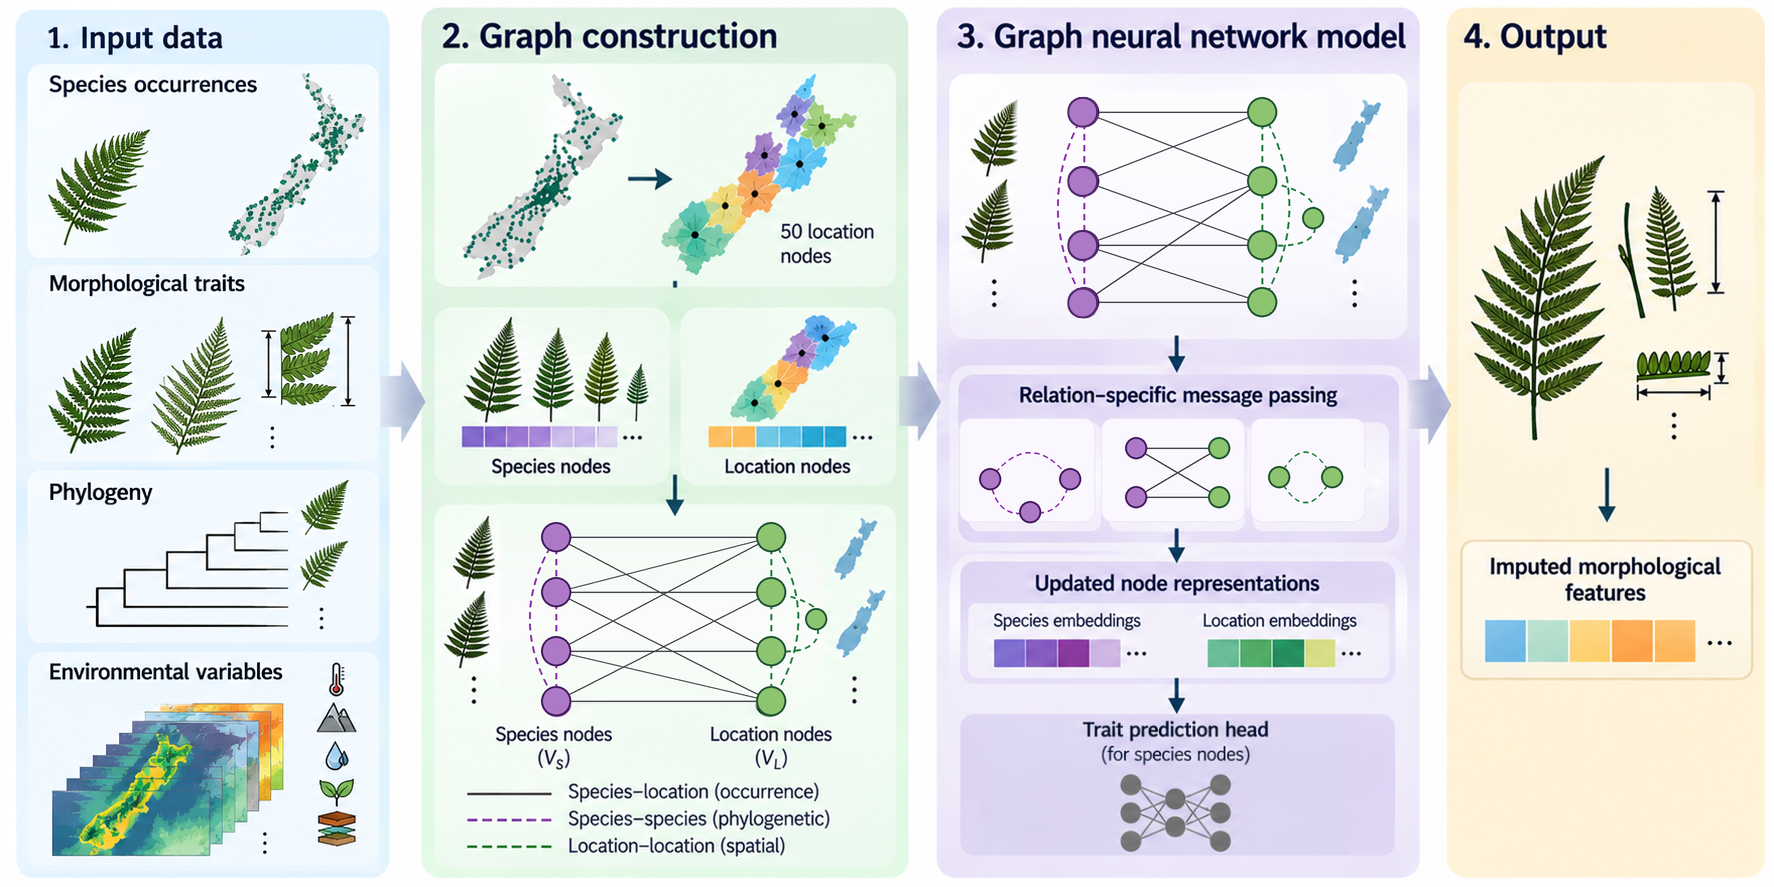
\includegraphics[width=\linewidth]{model pipeline.png}

\end{graphicalabstract}

%%Research highlights
\begin{highlights}
\item We introduce PhyEnv-NN, an integrated imputation framework to investigate the phylogenetic and environmental signal present in fern morphological traits.
\item The algorithm ranked first or second for 11 out of 12 outputs against baseline models commonly used in ecology.
\item Phylogenetic information provided the most consistent improvement in prediction accuracy.
\item Environmental predictors had limited aggregate effects but contributed to selected trait dimensions.
\item The framework allowed not only to fill missing trait values, but also to identify how biological information is structured across climates and phylogenies.

\end{highlights}

%% Keywords
\begin{keyword}
%% keywords here, in the form: keyword \sep keyword
trait variation; machine learning; ferns; trait predictability; variance structuring; phylogenetic signal; neural networks
%% PACS codes here, in the form: \PACS code \sep code

%% MSC codes here, in the form: \MSC code \sep code
%% or \MSC[2008] code \sep code (2000 is the default)

\end{keyword}

\end{frontmatter}

%% Add \usepackage{lineno} before \begin{document} and uncomment 
%% following line to enable line numbers
%% \linenumbers

%% main text
%%

\section{Introduction}
Explaining variation in morphological traits is central to understanding how species persist, evolve and diversify across ecological and climatic gradients \citep{adler_functional_2014,westoby_land-plant_2006}. Functional ecology has increasingly sought to organise plant variation into trait spectra and functional strategies that capture patterns of resource use, ecological interactions, and physiological and phenological variation \citep{diaz_global_2016, heilmeier2019functional, laughlin2023plant, majumder2024machine, mommer2012role, roddy2020towards, sanchezmartinez2020adaptation, walker2022functional, westoby1998leafheightseed, wright2004worldwide}. Trait variation is known to reflect the interplay between environmental conditions, evolutionary history and allometric constraints \citep{ciarle2025disentangling, flo2021climate, mencuccini2019leaf, niklas1994plant, sanchezmartinez2024framework}. However, while trait spectra describe how variation is organised, the extent to which different sources of biological and ecological information underpin that variation remains poorly understood \citep{caruso2020evolution}.

Some traits are evolutionarily labile and can respond strongly to environmental variation, leading to substantial divergence among closely related taxa \citep{ackerly2009conservatism, sanchezmartinez2024framework}. At the same time, the information carried by phylogenetic relatedness is inherently ambiguous. Closely related species may resemble one another because they share inherited traits, because they have experienced similar selective pressures, or because evolutionary responses are constrained by genetic correlations, limited genetic variation and other non-adaptive processes \citep{crisp2012phylogenetic, cruznicolas2025combination, gomulkiewicz2009demographic, wiens2010niche}. Consequently, trait similarity among related species cannot be straightforwardly attributed to phylogenetic conservatism, as natural selection may be equally responsible for the persistence of similarity across lineages \citep{westoby2007generalization}. 

Phylogenetic structure therefore represents potentially meaningful information about trait variation rather than a source of statistical dependence that can be removed without consequence \citep{laughlin2023plant}. Yet, conventional comparative approaches typically address phylogenetic structure either by incorporating it as a covariance structure or by correcting trait associations for shared ancestry \citep{felsenstein1985phylogenies, revell2022phylogenetic}. This typically requires phylogenetic information to be treated as evidence of a particular evolutionary process \citep{revell2022phylogenetic}. An alternative approach would be to treat phylogeny as a potential source of predictive information and directly test whether its inclusion improves the prediction of trait variation. Comparing predictive performance with and without phylogenetic and environmental information could quantify where trait variation is concentrated, without requiring that phylogenetic similarity be interpreted a priori as either shared ancestry or adaptation.

This idea can be operationalised by representing the available information as a heterogeneous graph. Species and sampled locations can be treated as distinct node types, with species occurrences defining links between them, following the general concept of species–habitat bipartite networks~\citep{marini_specieshabitat_2019,harrell2025heterogeneous}. Phylogenetic relationships provide an additional set of links among species, resulting in a graph in which trait information, environmental conditions, species distributions, and phylogenetic relationships are represented within a common relational structure. Graph neural networks can exploit this structure by propagating information along the different types of edges, allowing predictions for each species to incorporate information from both its phylogenetic relatives and the environments in which it occurs~\citep{bronstein2021geometric}.

In this study, we developed a graph-based machine learning framework to quantify the distribution of predictive information underlying trait variation in New Zealand ferns. First, we evaluated the predictive accuracy and reliability of the framework against established trait-prediction methods. We then systematically varied the phylogenetic, environmental and morphological information available to the model and quantified how prediction changed when each source of information was added or removed. By treating changes in predictive performance as evidence of incremental information, we tested the extent to which phylogenetic relationships and environmental conditions improve predictions of fern morphology and how these effects are structured across the fern phylogeny and morphological trait space.

\section{Methods}
\subsection{Data collection}
The fern flora of New Zealand was used  as a case study. This system constitutes a phylogenetically diverse flora distributed across strong environmental gradients \citep{mountier2018patterns}. It also provides a suitable test of our approach because trait descriptions are available for most species and include information on intraspecific variation \citep{brownsey2014flora}, while comparatively well-resolved phylogenies provide detailed information on evolutionary relationships \citep{nitta2022open}.

The species list used for this study was based on the Flora of New Zealand Ferns and Lycophytes \citep{brownsey2014flora} and included all species native to New Zealand. Because ferns exhibit high intraspecific variation, we did not focus on mean trait values. Instead, we tried to predict the maximum and minimum recorded trait sizes across the common morphological range of the species (i.e. excluding outliers). We retrieved data on the maximum and minimum lengths of sterile and fertile fronds, sterile and fertile stipes and spore size. Sterile and fertile frond data were kept separate as several species in the dataset produce morphologically distinct reproductive fronds (e.g. Blechnaceae). For species with monomorphic fronds, the same value was used for both fertile and sterile traits. As additional information for the model, we also recorded species altitudinal ranges, habit (i.e. obligate or occasional epiphytic, lithophytic, terrestrial) and level of hybridization. All data was amassed from the Flora of New Zealand Ferns and Lycophytes \citep{brownsey2014flora}. When unavailable, we searched the New Zealand Plant Conservation Network \citep{nzpcn_website}, Flora of New Zealand Online \citep{flora_of_nz_website} or the available scientific literature.

Phylogenetic information was based on the continuously updated fern tree of life (FTOL) \citep{nitta2022open}. Because discrepancies exist between the New Zealand and the International accepted nomenclature, we first used the Plants Of the World Online portal \citep{powo} to check for synonymity across our species list. We then used the R package \textit{ftolr} \citep{nitta2022open} to obtain a phylogenetic tree for our species by pruning the FTOL tree, which contains 5,582 out of the approximately 12,000 extant fern species. If a species was not present in FTOL but belonged to a genus present in the pruned tree, the species was coded as equally related to all species within the same genus. If a species was not present in FTOL and belonged to a genus absent in the pruned tree, the species was coded as equally related to all species within the same family. We avoided placing the missing species on the tree based on morphological similarity as that would defy the aim of the study.

Occurrences for each species were downloaded from the Global Biodiversity Information Facility \citep{gbif}, using the R package \textit{rgbif} \citep{chamberlain2017package}. These were then screened using the R package \textit{rnaturalearth} \citep{south2017r} to remove all occurrences that fell outside the New Zealand North, South and Stewart Islands and the 11 oceanic islands surrounding them \citep{ciarle2023island}. We only kept occurrences within the New Zealand region because this allowed us to have a well-defined study system both geographically and climatically, and because the morphological variability of each species was mainly recorded from specimens within the New Zealand region. We used the \textit{CoordinateCleaner} R package \citep{zizka2019coordinatecleaner} to avoid pseudoreplication, duplicated data points (i.e. multiple presence data points within 10' x 10' grid cells), and erroneous records (e.g. those occurring over ocean surfaces and cities). Since GBIF had no records for 7 New Zealand species (i.e. \textit{Hymenophyllum polyanthos}, \textit{Dicranopteris linearis}, \textit{Macrothelypteris torresiana}, \textit{Nephrolepis brownii}, \textit{Hymenophyllum falklandicum}, \textit{Botrychium lunaria}, and \textit{Arachniodes aristata}), we manually retrieved climatic information for those species based on their recorded range following the Flora of New Zealand Ferns and Lycophytes \citep{brownsey2014flora}. 

Because occurrences for threatened species were not readily available, they were retrieved from the WELT and AK herbaria records. Since WorldClim2 provides no information before 1970 \citep{fick2017worldclim}, all herbaria specimens collected prior to 1970 were not considered. Because GBIF occurrences tend to be geographically biased, with certain regions (e.g. the Wellington city region) being overrepresented compared to others, we used population density as a way of weighting occurrences and climatic distributions. Population density layer for the New Zealand region was downloaded from WorldPop \citep{tatem2017worldpop} at 30 arc resolution. 

Based on the cleaned species occurrences, we obtained climatic data for annual mean temperature and precipitation (AMT and AMP, respectively), mean diurnal and annual temperature range, precipitation seasonality, solar radiation, and water vapour pressure from WorldClim2 \citep{fick2017worldclim} at 2.5 minutes of resolution using the R package \textit{raster} \citep{hijmans2010raster}. Climatic data for each species was then transformed into a raster object using the packages \textit{raster} and \textit{terra} \citep{hijmans2022package}. We also obtained layers for ecosystem types and soil parameters (i.e. chemical limitation to plant growth, quantity of calcium and phosphorus in the soil, soil age, hardness, drainage capacity, particle size and pH) for the New Zealand region from the Manaaki Whenua Landcare Research Land Resource Information System portal \citep{LRIS}.

\subsection{Problem definition}

The task of predicting unknown species traits from available ones can be formalised as an imputation problem.
Let $\mathcal{S}$ denote the set of species and let $\mathcal{J}$ denote the set of morphological traits. The trait observations can be represented by a partially observed matrix
\begin{equation}
    Y \in \mathbb{R}^{|\mathcal{S}|\times|\mathcal{J}|},
\end{equation}
where $Y_{sj}$ is the value of trait $j$ for species $s$. We define the observation mask
\begin{equation}
    O_{sj}=\begin{cases}
        1, & \text{if }Y_{sj}\text{ is observed},\\
        0, & \text{otherwise}.
    \end{cases}
\end{equation}
Species--trait pairs unavailable after data acquisition are marked with $O_{sj}=0$. Additionally, each trait value is represented by its minimum and maximum recorded values. We use $v\in\{\min,\max\}$ to index these two output components and write the corresponding target as $Y_{s,j,v}$.

Unlike regression or classification tasks, which define a precise set of inputs and outputs, the predictive target to impute can be any entry of the matrix, with the available ones as inputs.
The task is therefore to learn an imputation function that predicts the unobserved part of the trait matrix from the observed traits and the relational and covariate information:
\begin{equation}
    \hat{Y}_{s,j,v}=f_{\theta}\left(Y,\hat O\right)_{s,j,v},
    \qquad O_{sj}=0,
\end{equation}
where $\hat O$ is the visibility mask used to train and evaluate the model on known measurements. This mask is built to have $\hat O_{sj}=0$ either when $O_{sj}=0$ or with a define probability $\rho$. In our particolar setting, $f_\theta$ can also contain additional features, such as environmental and physiological information.


The species phylogenetic descriptors, occurrence records, and environmental variables provide then additional information to recover the missing entries. To take advantage of this additional information, we designed a geometry-based deep learning algorithm to connect species based on their phylogenetic affinity, using recorded occurrences to incorporate environmental information.  

\subsection{Graph construction}
We represented the data described above as a weighted heterogeneous graph
$\mathcal{G}=(\mathcal{V},\mathcal{E})$. Its node set is the disjoint union
$\mathcal{V}=\mathcal{V}_{S}\mathbin{\dot\cup}\mathcal{V}_{L}$, where
$\mathcal{V}_{S}$ contains one node for each fern species and
$\mathcal{V}_{L}$ contains nodes representing locations. The graph has three
edge sets,
\begin{equation}
    \mathcal{E}=\mathcal{E}_{SL}\mathbin{\dot\cup}
    \mathcal{E}_{SS}\mathbin{\dot\cup}\mathcal{E}_{LL},
\end{equation}
with occurrence edges $\mathcal{E}_{SL}\subseteq
\mathcal{V}_{S}\times\mathcal{V}_{L}$, phylogenetic edges
$\mathcal{E}_{SS}\subseteq\mathcal{V}_{S}\times\mathcal{V}_{S}$, and spatial
neighbourhood edges $\mathcal{E}_{LL}\subseteq
\mathcal{V}_{L}\times\mathcal{V}_{L}$. Thus,
$\mathcal{B}=(\mathcal{V}_{S}\mathbin{\dot\cup}\mathcal{V}_{L},
\mathcal{E}_{SL})$ is the species--location bipartite graph at the core of the
representation, while $\mathcal{E}_{SS}$ and $\mathcal{E}_{LL}$ encode
relations within its two node types.

To construct the location nodes, the union of all species-distribution rasters
was aggregated to a $0.1^{\circ}$ grid and its occupied cells were partitioned
into 50 spatial clusters by spectral clustering. This prevents the creation of spatially isolated location nodes with few or no species occurrences and reduces the number of location nodes to a manageable size for the neural network. We opted for 50 clusters as a compromise between the number of location nodes and the number of species occurrences per node, based on a knee analysis of the cluster-size distribution.
Each location node was placed
at the centroid of a cluster and assigned the climatic, population-density,
elevation, ecosystem, and soil variables introduced above, averaged over the
cluster as node features $X_{\text{L}}$. Location nodes were connected to their six nearest spatial neighbours;
the corresponding edge weight was the Euclidean distance between each cluster
centroid. A species node was connected to a location node whenever the
species occurred in at least one grid cell assigned to that cluster. The weight
$w_{sl}$ of this edge was the normalized occurrence summed over those cells, thereby
retaining information on the spatial support of species $s$ within location
cluster $l$.

The phylogenetic subgraph was constructed from pairwise evolutionary distances between species in the FTOL tree pruned to the study species. Species pairs with distances below the median pairwise distance were connected, with the distance retained as the edge weight.
In addition, the complete tree, including its internal nodes,
was embedded with node2vec~\citep{grover2016node2vec} to obtain a 16-dimensional phylogenetic descriptor $X_\text{phy}$ for every species represented in the tree. 
Species absent from the tree were retained as isolated species nodes with a zero phylogenetic descriptor. Each species node also carried its available morphological trait values $X_\text{morph}$ expressed as the minimum and maximum recorded values for each trait. Missing trait entries were stored as zeros together with an explicit binary missingness mask, so that zero-filled values were never interpreted as observations. Finally, the one-hot-encoded categorical attributes (habitat, hybridisation, and family) $X_\text{cat}$ were included. The complete species feature vector was the concatenation of these three components, $X_\text{S} = [X_\text{morph}, X_\text{phy}, X_\text{cat}]$.
This construction places morphology, phylogenetic proximity, environmental conditions, and
geographic occurrence in a single relational object, allowing information to
be propagated between a species and both its relatives and the environments in
which it occurs.
\subsection{Neural network model}

\begin{figure}
    \centering
    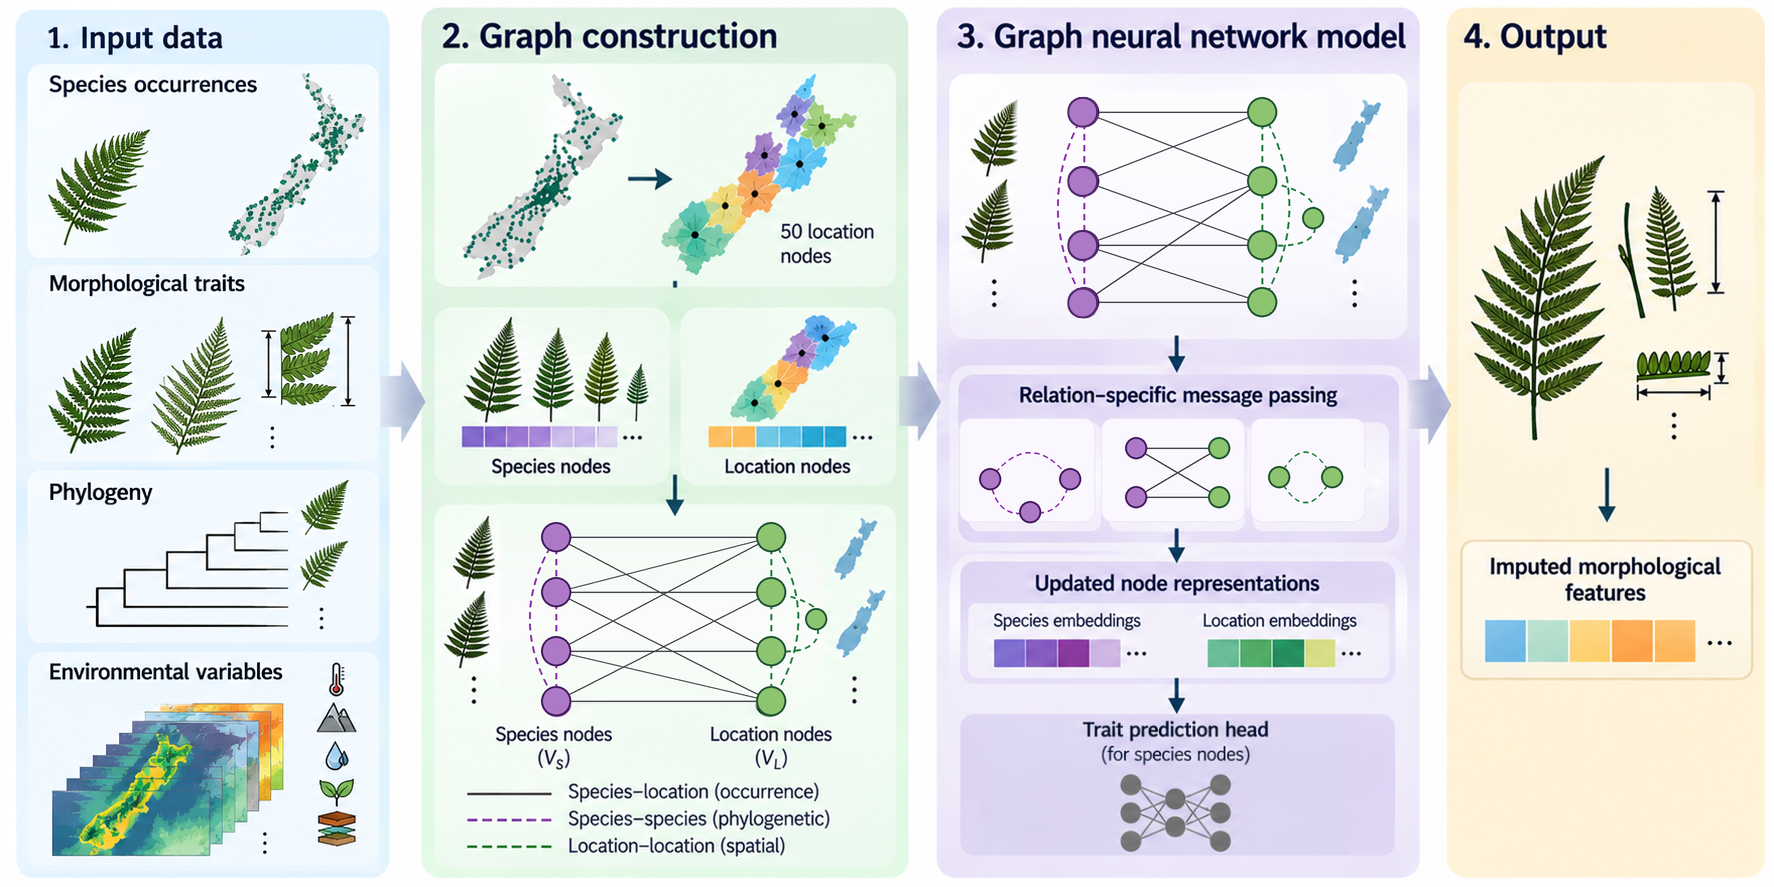
\includegraphics[width=\linewidth]{model pipeline.png}
    \caption{Visual description of the model's pipeline, including data used in input, graph construction and how different data sources are managed by the model.}
    \label{fig:model-pipeline}
\end{figure}
The \awesomeModel operates on the heterogeneous graph
\begin{equation}
    \mathcal{G}=
    (\mathcal{V}_{S}\mathbin{\dot\cup}\mathcal{V}_{L},
    \mathcal{E}_{SS}\mathbin{\dot\cup}\mathcal{E}_{LL}
    \mathbin{\dot\cup}\mathcal{E}_{SL}),
\end{equation}
where species nodes are connected through phylogenetic edges, location nodes through spatial-neighbourhood edges, and species and locations through occurrence edges. The model predicts missing species traits by combining the observed attributes of each species with information propagated through the spatial, occurrence, and phylogenetic relations.

More generally, the model can be viewed as a sequence of relation-specific transformations. We denote these transformations by \(f_{\theta}^{(\cdot)}\), where the superscript identifies their role in the model. Below, we first define each transformation generically and then specify the particular neural-network architecture used in our implementation.

\paragraph{Species encoder}

Let \(\hat O_s\) denote the visibility mask for species \(s\), which extends the $s^{th}$ row of the observation matrix $O$ by setting to zero both missing and intentionally masked trait values. We define the species input as the masked version of the corresponding species feature vector $X_\mathrm{S}$:
\begin{equation}
    x_s^{\mathrm{S}}
    =
    [
        X_{\mathrm{morph},s} \odot \hat O_s,
        \hat O_s,
        X_{\mathrm{phy},s},
        X_{\mathrm{cat},s}
        ],
\end{equation}
where \(X_{\mathrm{morph},s}\), \(X_{\mathrm{cat},s}\), and \(X_{\mathrm{phy},s}\) contain the morphological traits, categorical attributes, and phylogenetic descriptor for species $s$, respectively.
The visibility mask $\hat O_s$ is used both to mask unavailable trait values and as an explicit input feature, allowing the model to distinguish missing or intentionally masked entries from valid trait values that are zero after normalization.

The initial species representation is obtained as
\begin{equation}
    h_s^{\mathrm{S}}
    =
    f_{\theta_{\mathrm{S}}}
    \left(x_s^{\mathrm{S}}\right).
\end{equation}

In our implementation, \(f_{\theta_{\mathrm{S}}}\) is a linear projection with ReLU activation function.
This encoder therefore transforms the heterogeneous species-level inputs into a common latent representation without yet exchanging information between species.

\paragraph{Spatial encoder}

Each location \(l\) is described by its environmental covariates \(X_{L,l}\) and a positional encoding \(P_l\) of its latitude and longitude. We denote the corresponding input by
\begin{equation}
    x_l^{\mathrm{L}}=[X_{L,l},P_l].
\end{equation}
Information is propagated among neighbouring locations according to
\begin{equation}
    h_l^{\mathrm{L}}
    =
    f_{\theta_{LL}}
    \left(
        x_l^{\mathrm{L}},
        \mathcal{N}_{LL}(l),
        \{e_{ll'}\}
    \right),
\end{equation}
where \(\mathcal{N}_{LL}(l)\) denotes the spatial neighbours of location \(l\), and \(e_{ll'}\) denotes the attributes associated with their spatial edge.

We instantiate \(f_{\theta_{LL}}\) as a multilayer graph-attention network (GAT) with ReLU activations operating on the location--location graph \(\mathcal{E}_{LL}\). Thus, the representation of a location depends both on its own environmental conditions and on those of neighbouring spatial regions.

\paragraph{Species--location message passing}

The spatial representations are then transferred from location nodes to species nodes through the occurrence graph \(\mathcal{E}_{SL}\). To prevent trait values from directly influencing this spatial aggregation, the destination-side representation used at this stage excludes morphological traits. We therefore define
\begin{equation}
    q_s=[X_{\mathrm{cat},s},X_{\mathrm{phy},s}].
\end{equation}

The spatial information associated with species \(s\) is obtained through the relation-specific transformation
\begin{equation}
    b_s
    =
    f_{\theta_{LS}}
    \left(
        q_s,
        \{h_l^{\mathrm{L}}:
        l\in\mathcal{N}_{SL}(s)\},
        \{e_{sl}\}
    \right),
\end{equation}
where \(\mathcal{N}_{SL}(s)\) is the set of location nodes connected to species \(s\), and \(e_{sl}\) contains the occurrence-edge information.

In our implementation,
\(f_{\theta_{LS}}\)
is a GAT layer on the bipartite species--location graph. Learnable attention weights enable different locations to contribute differently to the environmental representation of a species.

The resulting spatial representation is then combined with the species encoding:
\begin{equation}
    \tilde h_s
    =
    [h_s^{\mathrm{S}},b_s].
\end{equation}
Importantly, \(h_s^{\mathrm{S}}\) is the only component of this representation that contains morphological trait values.

\paragraph{Phylogenetic species message passing}

The fused species representations are propagated through the species--species graph so that information can be exchanged between phylogenetically related species:
\begin{equation}
    h_s^{\mathrm{final}}
    =
    f_{\theta_{SS}}
    \left(
        \tilde h_s,
        \{\tilde h_{s'}:
        s'\in\mathcal{N}_{SS}(s)\},
        \{e_{ss'}\}
    \right),
\end{equation}
where \(\mathcal{N}_{SS}(s)\) contains the phylogenetic neighbours of species \(s\), and \(e_{ss'}\) contains their evolutionary-distance information.

We instantiate
\(f_{\theta_{SS}}\)
as a multilayer GAT with ReLU activations, using evolutionary distance as an edge attribute.


Finally, the latent representation of each species is mapped to its predicted morphological traits:
\begin{equation}
    \hat{\mathbf{Y}}_s
    =
    f_{\theta_{\mathrm{out}}}
    \left(h_s^{\mathrm{final}}\right).
\end{equation}

In our implementation, \(f_{\theta_{\mathrm{out}}}\) is a linear output layer where the two output blocks contain the predicted normalized minimum and maximum values, respectively, for each morphological trait.

\paragraph{Training objective}

The network is trained as a denoising masked reconstruction model. Let \(O\in\{0,1\}^{S\times J}\) denote the observation mask, with \(O_{s,j}=1\) when trait \(j\) is available for species \(s\) and \(O_{s,j}=0\) when it is genuinely missing. During training, a second binary mask \(\hat O\in\{0,1\}^{S\times J}\) is applied to the morphological input, such that

\[
    \widetilde X_{\mathrm{morph}}
    =
    X_{\mathrm{morph}}\odot \hat O ,
\]

where \(\hat O_{s,j}=0\) indicates that an observed species--trait entry is intentionally hidden from the model, whereas \(\hat O_{s,j}=1\) leaves it visible. For genuinely missing entries, \(O_{s,j}=0\) and \(\hat O_{s,j}=0\).

The reconstruction weight associated with each species--trait pair is defined as

\begin{equation}
    w_{s,j}
    =
    O_{s,j}
    \left[
        (1-\hat O_{s,j})
        +
        0.2\,\hat O_{s,j}
    \right].
\end{equation}

Thus, genuinely missing entries receive zero weight, observed entries intentionally masked from the input receive unit weight, and observed entries that remain visible receive weight \(0.2\). Let $W=\sum_{s=1}^{S}\sum_{j=1}^{J}w_{s,j}$. The reconstruction objective is

\begin{equation}
    \mathcal{L}_{\mathrm{recon}}
    =
    \frac{1}{2W}
    \sum_{s=1}^{S}\sum_{j=1}^{J}w_{s,j}
    \sum_{v\in\{\min,\max\}}
    \ell_{\mathrm{Huber}}\!\left(
        \hat{Y}_{s,j,v},Y_{s,j,v}
    \right).
    \label{eq:loss}
\end{equation}

Here, $Y_{s,j,v}$ is the observed component of $X_{\mathrm{morph}}$, and $\hat{Y}_{s,j,v}$ is its reconstructed value. The factor $2W$ averages the Huber error over the two output components and the weighted species--trait pairs. Species--trait pairs with genuinely missing observations make no contribution to the loss.

The \awesomeModel pipeline supports inference on species not seen during training. Provided that the required features can be constructed, new species can be added to the heterogeneous graph and their traits reconstructed without re-estimating the model parameters.


\subsection{Model explainability}

%%%%%%

To identify which biological and environmental variables contributed to the predicted distribution of each species, we interpreted the trained model using Integrated Gradients (IG). 
IG compares the model's response to the observed input with its response to a baseline input. The observed input $\mathbf{x}$ is the feature configuration for which an explanation is sought, whereas the baseline $\mathbf{x}'$ represents a reference configuration corresponding to the absence, or neutral level, of the information carried by those features. 
In our setting, $\mathbf{x}$ comprises the model inputs for all species and location nodes: $X_{\mathrm{morph}}$, $X_{\mathrm{phy}}$, and $X_{\mathrm{cat}}$ for species, and $X_{\mathrm{L}}$ for locations. The visibility mask $\hat O$ is held fixed during attribution, as are the graph structure and its species--location, species--species, and location--location connections. The model output is the reconstructed morphological feature tensor, with $\hat{Y}_{s,j,v}$ denoting the prediction for species $s$, trait $j$, and $v\in\{\min,\max\}$.

IG attributes the change in a given prediction between \(\mathbf{x}'\) and \(\mathbf{x}\) to the individual input variables by integrating their gradients along the straight-line path connecting the two inputs. For a scalar input variable \(x_k\), its attribution to \(\hat{Y}_{s,j,v}\) is

\begin{equation}
    \mathrm{IG}^{(s,j,v)}_k
    =
    (x_k-x'_k)
    \int_0^1
    \frac{\partial \hat Y_{s,j,v}
    \left(
    \mathbf{x}'+
    \alpha(\mathbf{x}-\mathbf{x}')
    \right)}
    {\partial x_k}
    \,d\alpha ,
\end{equation}

where \(x_k'\) is its corresponding value in the baseline input, and \(\alpha\in[0,1]\) parametrizes the interpolating line. Depending on $k$, $\mathrm{IG}^{(s,j,v)}_k$ therefore quantifies the contribution of an observed morphological feature, a component of a species phylogenetic representation, or an environmental feature associated with a location node to the predicted trait value of species \(s\).

We selected IG because it provides feature-level attributions for differentiable nonlinear models, making it particularly suited to disentangling the contribution of the heterogeneous biological and environmental predictors considered here. Related applications have used IG to identify taxonomically informative morphological features in orchid biodiversity monitoring and species invasiveness \citep{sangiovanni2025orchid,SPINA2026103877} and to quantify the contribution of spectral, climatic, and phenological variables in forest and vegetation modelling \citep{hiebl2026combining}. 

The integral was approximated numerically by evaluating the gradients at a sequence of points along the interpolation path, using a zero-valued baseline, i.e. setting \(\mathbf{x}'=\mathbf{0}\) for all input features.
Positive attributions indicate that, relative to the baseline, a variable contributes to increasing \(\hat{Y}_{s,j,v}\), whereas negative values indicate a contribution in the opposite direction; the absolute magnitude of the attribution reflects the strength of that contribution. Integrated Gradients were computed after training, with all model parameters held fixed, so that the resulting attributions characterise the behaviour of the fitted model rather than introducing an additional predictive component.


\subsection{Validation}
We first evaluated the models with a five-fold cross-validation at the species level. For each repetition, species were randomly assigned to five folds. Four folds were used for model fitting, and the remaining fold for evaluation, such that each species served as a test species exactly once within a complete cross-validation run. All preprocessing parameters, including transformations and scaling of morphological and environmental variables, were estimated exclusively from the outer-training species and subsequently applied using the corresponding fold-specific transformation. For model fitting, the graph was induced by the outer-training species, their phylogenetic edges, and their occurrence edges to the shared location nodes. Test-species traits and edges incident on test species therefore did not contribute to parameter estimation.

Model selection was separated from final evaluation by an additional validation mask constructed within each outer training fold. For each trait, \(15\%\) of its observed training entries were randomly withheld, subject to retaining at least one observation for training. Entries removed from the morphological input were retained as targets, and the model state with the lowest reconstruction loss within 1000 training epochs on this internal validation set was selected.
During model fitting, the visibility mask was formed as \(\hat O_{sj}=O_{sj}(1-R_{sj})\), where $R_{sj}=1$ identifies an observed entry intentionally hidden from the input. The corresponding morphological input was $\widetilde{X}_{\mathrm{morph}}=X_{\mathrm{morph}}\odot\hat O$, and the masked entries were reconstructed with the objective in Equation~\ref{eq:loss}. The same validation cells were used to fit trait-wise split-conformal residual bounds.

After the model training, final reconstruction performance was evaluated under a leave-one-trait-out procedure. For each target trait, both its minimum and maximum values were removed from the input of every species belonging to the outer test fold, while the remaining observed traits and non-morphological features of those species were retained. The fitted model was then used to reconstruct the withheld components. Thus, the evaluation measures the ability to infer an unavailable trait for a species from information available at prediction time, rather than reconstructing values visible to the model. Performance metrics were computed only for test species--trait pairs for which an original observation was available. Genuinely missing entries, for which no reference value existed, were excluded from evaluation. Within each repetition, predictions from the five outer folds were combined so that each evaluated species--trait value originated from a fold in which that species had not contributed to model fitting. Fold-level statistics were subsequently aggregated according to the number of available observations for each trait and output variable.
% In particular, errors were pooled across folds before computing the corresponding cross-validation summary, while correlations were combined using a weighted Fisher transformation.

We then compared \awesomeModel performance against Training Mean and Training Median imputers, phylogeny-based nearest-neighbour (NN and KNN) approaches, and established statistical methods for missing-trait reconstruction (MICE, Rphylopars) \citep{van2011mice, goolsby2017rphylopars}. Training Mean and Training Median impute each missing trait component using respectively the mean or median estimated from the observed values of the outer-training species. Phylo NN and Phylo KNN use the original phylogenetic tree directly. For each missing trait component, Phylo NN assigns the value of the phylogenetically closest training species for which that component is observed, whereas Phylo KNN uses the unweighted mean of the five closest observed training species. Species not represented among the tips of the phylogenetic tree were excluded from these phylogeny-dependent analyses.

MICE was evaluated using the original R \textit{mice} package \citep{van2011mice}. Conditional imputations were performed using classification and regression trees, with the observed morphological variables and the categorical species attributes supplied to the imputer. The chained-equation model was fitted on the outer-training species and subsequently applied to the test species without refitting its specification on the held-out target values.

Similarly, Rphylopars was evaluated using the R package \textit{Rphylopars} \citep{goolsby2017rphylopars}. Missing trait values were reconstructed using a Brownian-motion model of trait evolution, based on the phylogenetic tree and observed morphological traits. Because estimation of a fully correlated multivariate phylogenetic covariance was numerically unstable for the present trait set, the Brownian-motion model was fitted with a diagonal phylogenetic covariance. Evolutionary parameters, including the ancestral trait mean and phylogenetic covariance, were estimated from the outer-training species and kept fixed when reconstructing traits for held-out species.

To ensure consistency with our model evaluation, all baselines used the same outer species folds and the same leave-one-trait-out reconstruction scheme. Specifically, each baseline was first fitted using only the outer-training species. For each target trait, its minimum and maximum columns were then set to missing for all test species before applying the fitted imputer. Other observed traits of the same test species remained available whenever the baseline method could use them. The reconstructed minimum and maximum values for the target trait were retained, after which the procedure was repeated for every trait. This design prevented the true target values of held-out species from contributing to model fitting while preserving the information legitimately available for imputing that trait, thus matching the prediction setting used for \awesomeModel.

We used the same sequence of 60 random seeds for all models. For deterministic models, the seeds produced the same cross-validation results across different dataset splits. For nondeterministic models, the same splits were used, while the seeds also produced different parameter initializations. We conducted all the experiments using Python 3.12. PyTorch 2.12 was used for the graph models, together with \textit{rpy2} version 3.6 for the R-based baselines. The R baselines were run on R 4.5.3, using the corresponding original packages \citep{r2021r}.

To quantify prediction accuracy, normalized RMSE was calculated for each held-out trait-variable as the root mean squared reconstruction error on the original measurement scale divided by the interquartile range (IQR) of that trait-variable’s observed values across species. This expresses prediction error relative to the trait’s typical variation and allows comparisons across traits measured on different scales. Unlike min–max normalization, which uses only the two extremes of each trait's distribution and can be strongly affected by outliers, IQR normalization is robust to sensibly low or high observations. It therefore provided a more stable indication of error relative to the central distribution when comparing predictive performance or the improvement associated with additional model inputs.

Finally, to determine which type of information improved trait imputation, we performed an ablation analysis. To do so, we ran four \awesomeModel configurations: no additional inputs, environmental information only, phylogenetic information only, and both sources. We then compared their normalized RMSE-IQR at the trait level.

% Imputation error can also conflate model fit with estimation efficiency, meaning a model can win on prediction accuracy partly because it has fewer parameters to estimate from a noisy, masked sample, rather than because its assumptions are biologically closer to the truth. To control for this, for each model we measured the Akaike Information Criterion (AIC), which penalizes parameter count \citep{akaike2025akaike} If RMSE and AIC point the same direction for a trait, that can be considered a real biological signal. If they disagree, this may indicate that sample-size/estimation noise is playing a role. 

\subsection{Attribution analysis}

To highligth environmental feature importance in determining morphological dimension, we analysed IG attributions at the trait level. This allowed us to determine how the model distributed predictive information across environmental inputs. We used the absolute attribution magnitude because the analysis concerns the strength of model reliance on each input, independent of whether that input increases or decreases the predicted value. Trait-specific aggregation preserves differences in model behaviour that would be hidden by averaging across all prediction targets.

We also grouped environmental variables into broader input domains to compare the types of environmental information used by the model. The complete assignment of features to domains is reported in~\ref{app:features-domains}. Because the domains contained different numbers of variables, we report two complementary quantities. For a domain $d$ containing $N_d$ features, the mean absolute attribution is

\begin{equation}
    A_d =
    \frac{1}{N_d}
    \sum_{j \in d} \left|\mathrm{IG}_j\right|.
\end{equation}

This quantity measures the average attribution of a feature within the domain and therefore allows comparison between domains with different dimensionalities.

We also measured the fraction of total environmental attribution assigned to each domain. For domain $d$, the attribution share is

\begin{equation}
    S_d =
    \frac{
        \sum_{j \in d} \left|\mathrm{IG}_j\right|
    }{
        \sum_{k \in \mathcal{E}} \left|\mathrm{IG}_k\right|
    },
\end{equation}

where $\mathcal{E}$ denotes the set of environmental features. The attribution share measured the total amount of environmental attribution associated with a domain. Unlike $A_d$, this quantity depends on both the attribution magnitude of individual features and the number of features assigned to the domain. We therefore used $A_d$ to compare attribution strength across domains and $S_d$ to describe how the model distributed its total environmental attribution.

\subsection{Residuals analysis}

To map the distribution of predictive information, we analysed the structure of prediction residuals across both phylogeny and trait distributions. For each trait, we first calculated species-level residuals for all models. Model improvement was then quantified as the species-level reduction in prediction error, computed as

\begin{equation}
    \Delta_\mathrm{err} = \frac{|r_{m_I}| - |r_{m_{II}}|}{\mathrm{Observed\; trait\; value}}
\end{equation}

where $r$ denotes model residuals. 
$\Delta_\mathrm{err}$ was scaled by the corresponding observed trait value because absolute residual magnitude increased with the observed trait value in our predictions. The normalization therefore expresses model improvement relative to trait magnitude and limits the influence of this heteroscedastic error structure.
% $\Delta_\mathrm{err}$ were scaled by the corresponding observed trait values because neural networks are typically subject to a heteroskedasticity bias and naturally produce larger absolute errors for larger raw values. 
This scaling made the proportional error reductions apparent, i.e., the percentage of improvement relative to trait size. The model using more information was always put as the second term ($m_{II}$), so that positive values of {$\Delta_\mathrm{err}$} indicated improved prediction, whereas values less than or equal to zero indicate no improvement or reduced predictive performance.

To test whether prediction improvement was phylogenetically structured, we quantified the phylogenetic signal of each $\Delta_\mathrm{err}$ using the phylosig function in the R package phytools \citep{revell2024phytools}. The function returns a value of Pagel's $\lambda$. There is no phylogenetic signal when Pagel's $\lambda$ = 0. When Pagel's $\lambda$ = 1, there is evidence for a strong phylogenetic signal, indicating that trait evolution is compatible with a Brownian motion model, and trait differences can be reasonably well explained by phylogenetic distance. 

To then assess whether improvements in model predictive accuracy (i.e. $\Delta_\mathrm{err}$) were localized to specific evolutionary lineages, we calculated Local Moran's I for each species across all traits' $\Delta_\mathrm{err}$. Moran's I \citep{moran1950notes} is usually known as a measure of spatial autocorrelation in landscape ecology \citep{albassatneh2023effect}. However, in a phylogenetic context, it uses the phylogenetic proximity among species, instead of spatial proximity \citep{keck2016phylosignal}. While global phylogenetic signal metrics (e.g., Pagel's $\lambda$) measure trait conservatism across an entire phylogeny, local spatial statistics can identify specific tips or clades that deviate significantly from a global expectation of spatial independence \citep{anselin1995local}. Moran's I was calculated using the lipaMoran function in the R package phylosignal \citep{keck2016phylosignal}. Statistical significance was determined via a two-sided Monte Carlo permutation procedure (N = 999) against a null model of random tip shuffling. 

Tips exhibiting significant local autocorrelation (p < 0.05) were categorized into four groups: High-High (Hotspots): species with substantial predictive gains surrounded by relatives experiencing similar improvements; Low-Low (Coldspots): species exhibiting poor or negligible error reduction alongside phylogenetic neighbours of similar performance; High-Low / Low-High (Outliers): isolated species whose predictive performance was sharply higher (or lower) compared to that of their close evolutionary relatives.

Finally, to assess whether changes in prediction error varied across trait distributions, species were assigned to quantiles based on their observed trait values. We then compared $\Delta_\mathrm{err}$ among quantiles to determine whether prediction improvements were concentrated among species with relatively small, intermediate, or large trait values.

\section{Results}
\subsection{Reconstruction performance against baselines}

We gathered data for 208 fern species and subspecies, encompassing all of New Zealand's native flora. Of these, 174 were presented on the FTOL tree. Table~\ref{tab:performance_traits} compares the reconstruction performance of \awesomeModel with statistical, phylogenetic, and multivariate imputation baselines. \awesomeModel ranks first or second for 11 of the 12 output variables, getting the lowest NRMSE-IQR for five outputs. The only exception is minimum altitude, for which \awesomeModel ranks third behind training-median and training-mean imputation. This shows more consistent performance across traits than the competing methods.


\begin{table}[H]
\caption{Comparison of model performance based on NRMSE-IQR across independent benchmark seeds for the individual morphological traits. The best (lowest) value for each output variable is shown in bold, and the second-best value is underlined.}
\label{tab:performance_traits}
\resizebox{\textwidth}{!}{%
\begin{tabular}{lcccccccccccc}
\toprule
& \multicolumn{2}{c}{Altitude range} & \multicolumn{2}{c}{Fertile stipe length} & \multicolumn{2}{c}{Fertile frond length} & \multicolumn{2}{c}{Spore size} & \multicolumn{2}{c}{Sterile frond length} & \multicolumn{2}{c}{Sterile stipe length} \\
\cmidrule(lr){2-3} \cmidrule(lr){4-5} \cmidrule(lr){6-7} \cmidrule(lr){8-9} \cmidrule(lr){10-11} \cmidrule(lr){12-13}
\textbf{Model}
& \textbf{max} & \textbf{min} & \textbf{max} & \textbf{min} & \textbf{max} & \textbf{min} & \textbf{max} & \textbf{min} & \textbf{max} & \textbf{min} & \textbf{max} & \textbf{min} \\
\midrule

Training Mean & \bfseries 9.994 & \itshape \underline{0.790} & 1.754 & 0.736 & 2.449 & 0.936 & 18.571 & 16.312 & 2.450 & 0.931 & 1.822 & 0.750 \\
Training Median & 10.288 & \bfseries 0.787 & 1.798 & 0.775 & 2.529 & 0.969 & \bfseries 18.527 & \itshape \underline{16.271} & 2.536 & 0.961 & 1.867 & 0.793 \\
Phylo Nn & 12.518 & 0.925 & 1.803 & 0.606 & 1.813 & 0.643 & 18.777 & 16.490 & 1.818 & 0.660 & 1.862 & 0.634 \\
Phylo Knn & 11.163 & 0.807 & 1.769 & 0.549 & 1.748 & 0.656 & 18.831 & 16.549 & 1.752 & 0.658 & 1.835 & 0.562 \\
Mice & 10.284 & 0.986 & 1.824 & \bfseries 0.311 & 2.724 & 1.331 & 25.543 & 16.393 & 2.723 & 1.327 & 1.991 & \bfseries 0.323 \\
Rphylopars Bm & 10.940 & 0.805 & \itshape \underline{1.737} & 0.560 & \bfseries 1.605 & \itshape \underline{0.574} & 18.775 & 16.472 & \bfseries 1.609 & \itshape \underline{0.591} & \itshape \underline{1.801} & 0.584 \\

\midrule
\awesomeModel  (ours) & \itshape \underline{10.262} & 0.797 & \bfseries 1.518 & \itshape \underline{0.454} & \itshape \underline{1.662} & \bfseries 0.530 & \itshape \underline{18.534} & \bfseries 16.262 & \itshape \underline{1.723} & \bfseries 0.533 & \bfseries 1.551 & \itshape \underline{0.473} \\

\bottomrule
\end{tabular}
}
\end{table}

The competing methods performed well on narrower subsets of traits. MICE obtained the lowest error for minimum fertile and sterile stipe size, with NRMSE-IQR values of 0.311 and 0.323, respectively, but performed substantially worse on the frond variables and maximum spore size. Rphylopars performed best for maximum fertile and sterile frond size, reaching 1.605 and 1.609, respectively, and ranked second for several related variables. The phylogenetic nearest-neighbour methods improved over simple aggregation for some frond and stipe components but did not achieve the best score for any output. In contrast, \awesomeModel remained among the two best methods across frond, stipe, and spore traits.

Altitudinal range and maximum spore size were an exception. Simple training-set aggregation gave the best result for both altitude components: the training mean reached 9.994 for maximum altitude, and 0.787 for minimum altitude. The training median also gave the lowest error for maximum spore size at 18.527, only slightly below the 18.534 obtained by \awesomeModel. These results suggest that these evaluated predictors contain limited exploitable information for these outputs beyond their marginal distributions. The NRMSE-IQR values for these 2 traits also remained much larger than those of the other traits across all methods, further indicating that additional model complexity does not consistently improve reconstruction over simple mean or median imputation.

% \begin{table}
% \caption{Performance in terms of mean NRMSE-IQR across independent benchmark seeds for morphological traits and their output components. The best (lowest) value for each output variable is shown in bold, and the second-best value is underlined.}
% \label{tab:performance_traits}
% \resizebox{\textwidth}{!}{%
% \begin{tabular}{lcccccccccccc}
% \toprule
% & \multicolumn{2}{c}{Alt} & \multicolumn{2}{c}{Ferstipe} & \multicolumn{2}{c}{Fertile Frond} & \multicolumn{2}{c}{Spore} & \multicolumn{2}{c}{Sterile Frond} & \multicolumn{2}{c}{Sterile Stipe} \\
% \cmidrule(lr){2-3} \cmidrule(lr){4-5} \cmidrule(lr){6-7} \cmidrule(lr){8-9} \cmidrule(lr){10-11} \cmidrule(lr){12-13}
% \textbf{Model}
% & \textbf{max} & \textbf{min} & \textbf{max} & \textbf{min} & \textbf{max} & \textbf{min} & \textbf{max} & \textbf{min} & \textbf{max} & \textbf{min} & \textbf{max} & \textbf{min} \\
% \midrule
% Training Mean & \bfseries 9.994 ± 0.039 & \itshape \underline{0.790 ± 0.003} & 1.754 ± 0.006 & 0.736 ± 0.003 & 2.449 ± 0.009 & 0.936 ± 0.004 & 18.571 ± 0.009 & 16.312 ± 0.009 & 2.450 ± 0.009 & 0.931 ± 0.004 & 1.822 ± 0.006 & 0.750 ± 0.003 \\
% Training Median & 10.288 ± 0.000 & \bfseries 0.787 ± 0.001 & 1.798 ± 0.004 & 0.775 ± 0.003 & 2.529 ± 0.003 & 0.969 ± 0.005 & \bfseries 18.527 ± 0.004 & \itshape \underline{16.271 ± 0.003} & 2.536 ± 0.002 & 0.961 ± 0.007 & 1.867 ± 0.005 & 0.793 ± 0.002 \\
% Phylo Nn & 12.518 ± 1.186 & 0.925 ± 0.028 & 1.803 ± 0.042 & 0.606 ± 0.029 & 1.813 ± 0.176 & 0.643 ± 0.056 & 18.777 ± 0.053 & 16.490 ± 0.037 & 1.818 ± 0.175 & 0.660 ± 0.056 & 1.862 ± 0.044 & 0.634 ± 0.028 \\
% Phylo Knn & 11.163 ± 0.210 & 0.807 ± 0.019 & 1.769 ± 0.014 & 0.549 ± 0.012 & 1.748 ± 0.069 & 0.656 ± 0.021 & 18.831 ± 0.476 & 16.549 ± 0.417 & 1.752 ± 0.069 & 0.658 ± 0.022 & 1.835 ± 0.015 & 0.562 ± 0.013 \\
% Mice & 10.284 ± 0.123 & 0.986 ± 0.064 & 1.824 ± 0.382 & \bfseries 0.311 ± 0.040 & 2.724 ± 0.000 & 1.331 ± 0.000 & 25.543 ± 6.102 & 16.393 ± 0.025 & 2.723 ± 0.000 & 1.327 ± 0.000 & 1.991 ± 0.375 & \bfseries 0.323 ± 0.044 \\
% Rphylopars Bm & 10.940 ± 0.396 & 0.805 ± 0.020 & \itshape \underline{1.737 ± 0.015} & 0.560 ± 0.014 & \bfseries 1.605 ± 0.046 & \itshape \underline{0.574 ± 0.016} & 18.775 ± 0.048 & 16.472 ± 0.042 & \bfseries 1.609 ± 0.046 & \itshape \underline{0.591 ± 0.016} & \itshape \underline{1.801 ± 0.015} & 0.584 ± 0.015 \\

% \midrule
% \awesomeModel (ours) & \itshape \underline{10.262 ± 0.069} & 0.797 ± 0.014 & \bfseries 1.518 ± 0.076 & \itshape \underline{0.454 ± 0.024} & \itshape \underline{1.662 ± 0.387} & \bfseries 0.530 ± 0.050 & \itshape \underline{18.534 ± 0.025} & \bfseries 16.262 ± 0.023 & \itshape \underline{1.723 ± 0.525} & \bfseries 0.533 ± 0.054 & \bfseries 1.551 ± 0.094 & \itshape \underline{0.473 ± 0.025} \\
% \bottomrule
% \end{tabular}
% }
% \end{table}

\subsection{Ablation}

The ablation analysis showed that phylogenetic information provided the main improvement in trait imputation, whereas environmental information contributed little at the aggregate level. Across all trait--variable slices, the median NRMSE-IQR was 4.591 for the baseline, 4.595 with environmental information, 4.512 with phylogenetic information, and 4.511 with both. Thus, adding phylogenetic information reduced the median NRMSE-IQR by 0.079 relative to the baseline, while adding environmental information to the phylogeny-only model yielded a further reduction of only 0.002. Environmental information alone slightly increased the median error.

Figure~\ref{fig:ablation-contrast} shows that these effects varied substantially among traits, with the strongest benefits of additional information concentrated in frond dimensions. The most consistent improvement occurred when phylogenetic information was introduced. Relative to the baseline, it improved predictions of minimum and maximum fertile and sterile frond dimensions, as well as minimum altitude and minimum sterile stipe size. The largest gains were for minimum fertile and sterile frond size, for which phylogeny alone reduced NRMSE-IQR by 0.340 and 0.355, respectively. The same pattern emerged when phylogeny was added to the environment-only model, with reductions of 0.438 and 0.387 for these two traits. The full model likewise retained substantial improvements relative to the baseline (0.424 and 0.372, respectively). Overall, transitions introducing phylogenetic information produced the strongest gains, although their effects remained trait-dependent.

\begin{figure}[H]
    \centering
    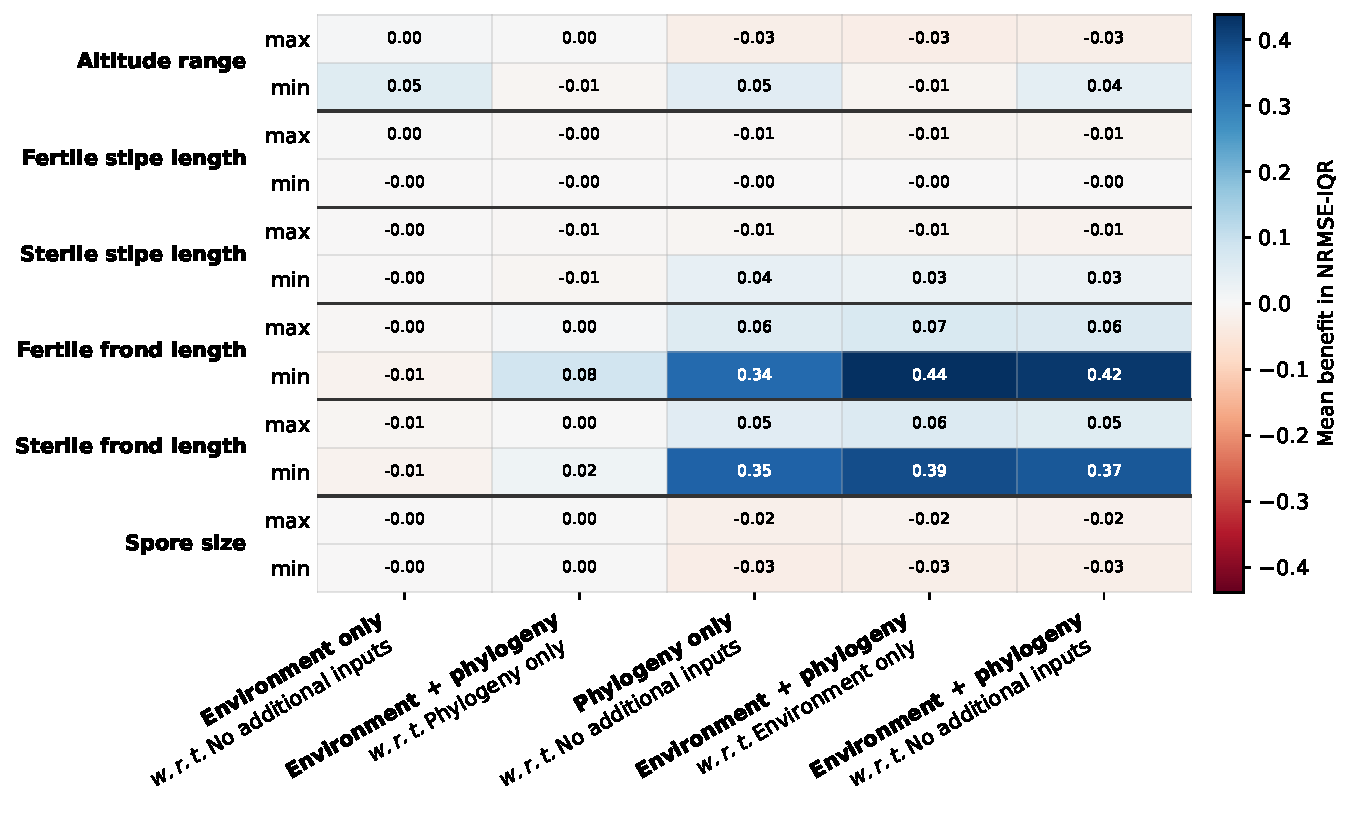
\includegraphics[width=.9\textwidth]{ablation_marginal_effects_slices.pdf}
    \caption{Mean change in prediction accuracy when environmental and phylogenetic information are added to the imputation model. Cells show the mean reduction in NRMSE-IQR for each trait under five model contrasts. Positive values (in blue) indicate that the model containing the added information (highlighted in bold) had lower prediction error than the reference model (written below); negative values (in red) indicate higher error. Phylogenetic information produced the largest mean improvements for minimum fertile and sterile frond length, whereas environmental predictors alone produced little average change across trait bounds.}
    \label{fig:ablation-contrast}
\end{figure}

Environmental information provided an additional benefit primarily for frond dimensions once phylogeny was included, reducing NRMSE-IQR by a further 0.084 for minimum fertile frond size and 0.018 for minimum sterile frond size. Aside from these traits, environmental information had little effect and sometimes reduced performance. Environment-only contrasts were close to zero for most trait--variable slices and were negative for minimum fertile and sterile frond size. Adding environmental information to the phylogeny-only model also produced only minor changes, but slightly worsened predictions for minimum altitude and both fertile and sterile stipe components, with contrast magnitudes below 0.01 except for minimum altitude $-0.009$. 

Spore size followed a different pattern: environmental information alone had almost no effect, whereas introducing phylogenetic information increased error for both its minimum and maximum components. Maximum altitude and the maximum fertile and sterile stipe dimensions likewise showed small negative contrasts when phylogeny was included. Overall, the ablation analysis showed that phylogenetic information carried most of the predictive signal, particularly for frond dimensions, while environmental information contributed little beyond phylogeny and instead slightly reduced performance for some altitudinal ranges and stipe traits.

\subsection{Attribution analysis}

Environmental attribution varied across target traits and individual features, so global feature averages masked part of the model's behaviour. Figure~\ref{fig:pertarget_attributions} therefore reports mean absolute integrated-gradient attribution separately for each trait--output component. Stipe and frond traits generally received larger environmental attributions than altitudinal range and spore traits, and also had the weakest reconstruction performance in Table~\ref{tab:performance_traits}, consistent with the environmental inputs carrying less predictive information for these targets.

Soil pH received the largest feature-level attribution across the evaluated environmental variables. Its maximum mean absolute attribution was $8.168\times10^{-3}$ for minimum sterile stipe size. This value was approximately 10\% larger than the second-highest attributed feature and 47\% above the mean attribution of the remaining environmental features for that target. The same pattern extended across the stipe and frond traits: soil pH attribution was, on average, approximately 39\% larger than the mean attribution of the other environmental features. Other environmental variables showed stronger attribution only for selected targets, indicating that the model did not rely on a common environmental profile across traits.

\begin{figure}[ht]
    \centering
    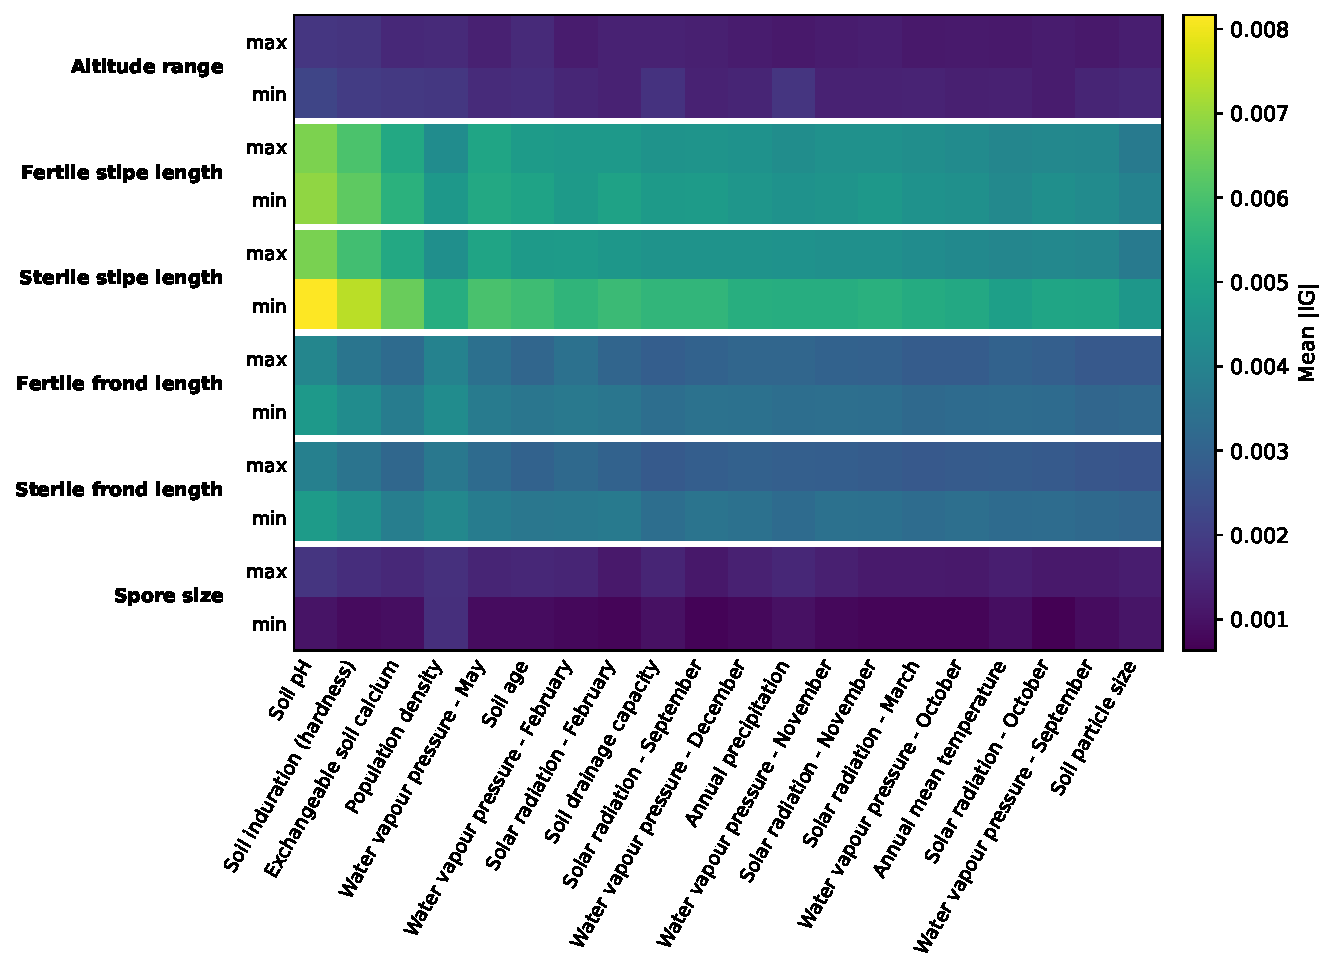
\includegraphics[width=0.8\linewidth]{env_feature_target_heatmap.pdf}
    \caption{Mean absolute integrated-gradient (IG) attribution of environmental predictors across trait targets. Rows represent minimum and maximum trait values, and columns show the environmental variables with the highest overall attribution. Colours indicate mean absolute integrated-gradient values, with higher values denoting a greater contribution of a predictor to the corresponding model output.}
    \label{fig:pertarget_attributions}
\end{figure}

The domain-level analysis (Figure~\ref{fig:domain_attributions}) revealed how climate accounted for approximately 68\% of total environmental attribution across traits, soil accounted for approximately 21\%, and elevation for approximately 3\%. Their magnitude also reflected the unequal number of variables in each domain: climate contains 29 features, soil contains 10, and elevation contains one. Domain attribution share therefore measures how the model distributes total environmental attribution, but it does not directly compare the attribution strength of an individual feature from each domain.

Mean absolute attribution per feature revealed stronger differences among traits and domains. Altitudinal range and spore traits had low mean attribution across all environmental domains, matching the feature-level pattern in Figure~\ref{fig:pertarget_attributions}. Soil variables received their strongest mean attribution for stipe-related targets, with the largest values for sterile stipe components. Climate variables contributed a large fraction of total environmental attribution but had lower attribution per feature: for stipe- and frond-related traits, their mean attribution was approximately 24\% lower than that of soil variables. Elevation had the lowest mean attribution across the evaluated traits.

\begin{figure}[ht]
    \centering
    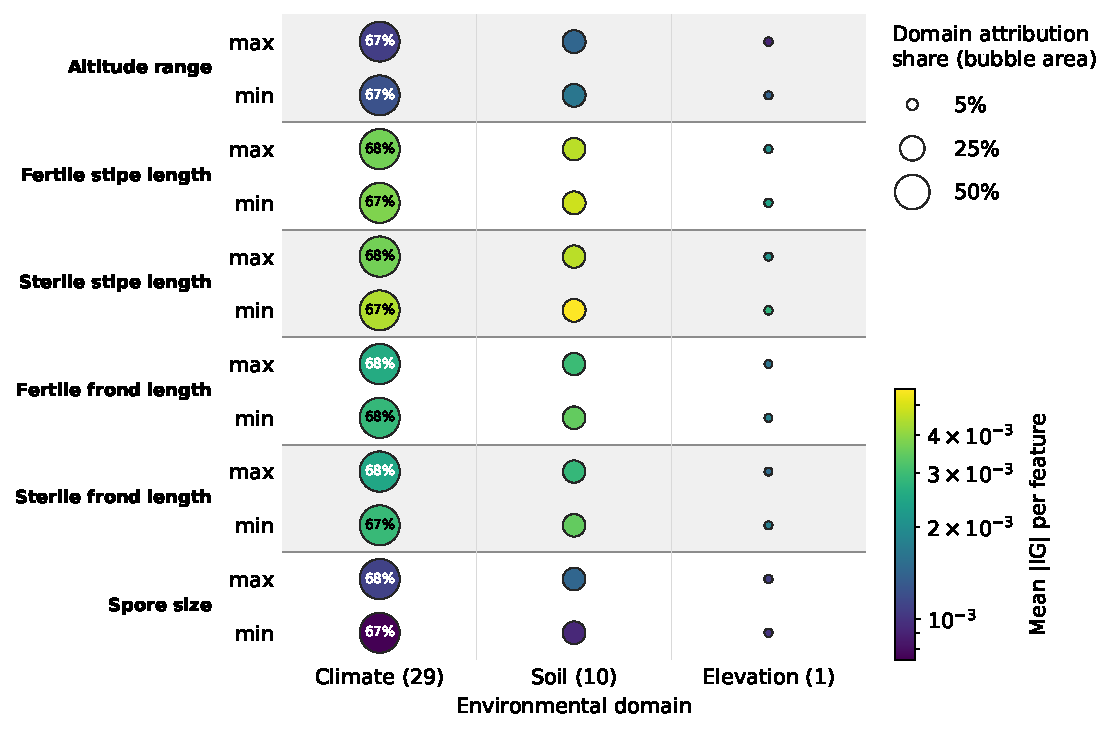
\includegraphics[width=0.8\linewidth]{env_domain_bubble_matrix.pdf}
    \caption{Environmental attribution across predictor domains and trait targets. Circle area represents the proportion of total absolute integrated-gradient (IG) attribution assigned to each environmental domain. Circle colour indicates the mean absolute attribution per feature within each domain. Climate variables accounted for the largest share of total environmental attribution across all targets, largely because this domain contained 29 predictors, whereas soil variables had the highest per-feature attribution.}
    \label{fig:domain_attributions}
\end{figure}

\subsection{Residuals analysis}

The species-level error analysis showed that the benefit of additional information was also structured across the phylogeny. Most proportional delta improvements ($\Delta_\mathrm{err}$) were phylogenetically structured across fertile and sterile frond length, and to a lesser degree across altitudinal range, but not across fertile and sterile stipe length and spore size. (Figure~\ref{fig:lambda}). However, Moran's I revealed that phylogenetic information improved trait imputation in a lineage-dependent manner. Improvements in $\Delta_\mathrm{err}$ were concentrated in maximum fertile and sterile frond length and spore size, suggesting that these traits retain stronger lineage-level structure than the other measured traits Figure~\ref{fig:moransI}. 

\begin{figure}
    \centering
    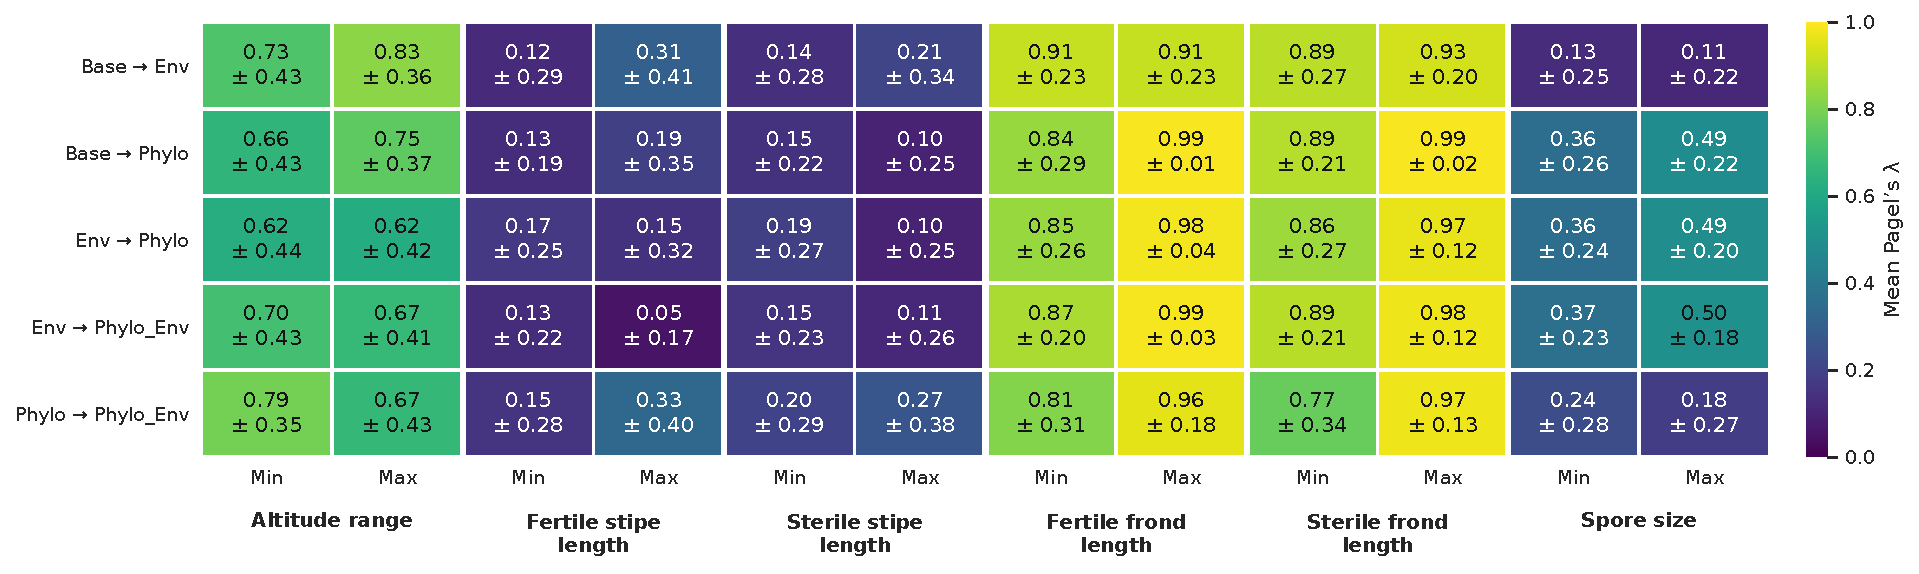
\includegraphics[width=1\linewidth]{Lambda signal.pdf}
    \caption{Phylogenetic signal of prediction-error changes associated with transitions between model configurations. Rows indicate the addition of environmental (Env) and phylogenetic (Phylo) information relative to the baseline (Base) or to a model already containing one information source. Columns represent the six morphological traits' minimum and maximum values. Higher values indicate that a $\Delta_\mathrm{err}$ is clustered across the phylogeny.}
    \label{fig:lambda}
\end{figure}

For maximum fertile frond length, species of \textit{Tmesipteris} (family Psilotaceae) repeatedly formed hotspots (i.e. phylogenetic regions with substantial predictive gains surrounded by relatives experiencing similar improvements) when phylogenetic information was included. In the Base $\rightarrow$ Phylo transition, \textit{Tmesipteris sigmatifolia} was a hotspot in 92\% of seeds, and \textit{T. horomaka} was a hotspot in 85\% of seeds. In the Env $\rightarrow$ Phylo transition, \textit{T. sigmatifolia} remained a hotspot in 90\% of seeds. The Env $\rightarrow$ Phylo\_Env comparison similarly identified \textit{T. sigmatifolia} as a hotspot in 93\% of seeds and \textit{T. tannensis} as a hotspot in 85\% of seeds. In contrast, \textit{Azolla rubra} was identified as a Low--High outlier for maximum fertile frond length in 80\% to 85\% of seeds, meaning its predictive performance was sharply or lower compared to that of its close evolutionary relatives (Figure~\ref{fig:moransI}).

\begin{figure}[ht]
    \centering
    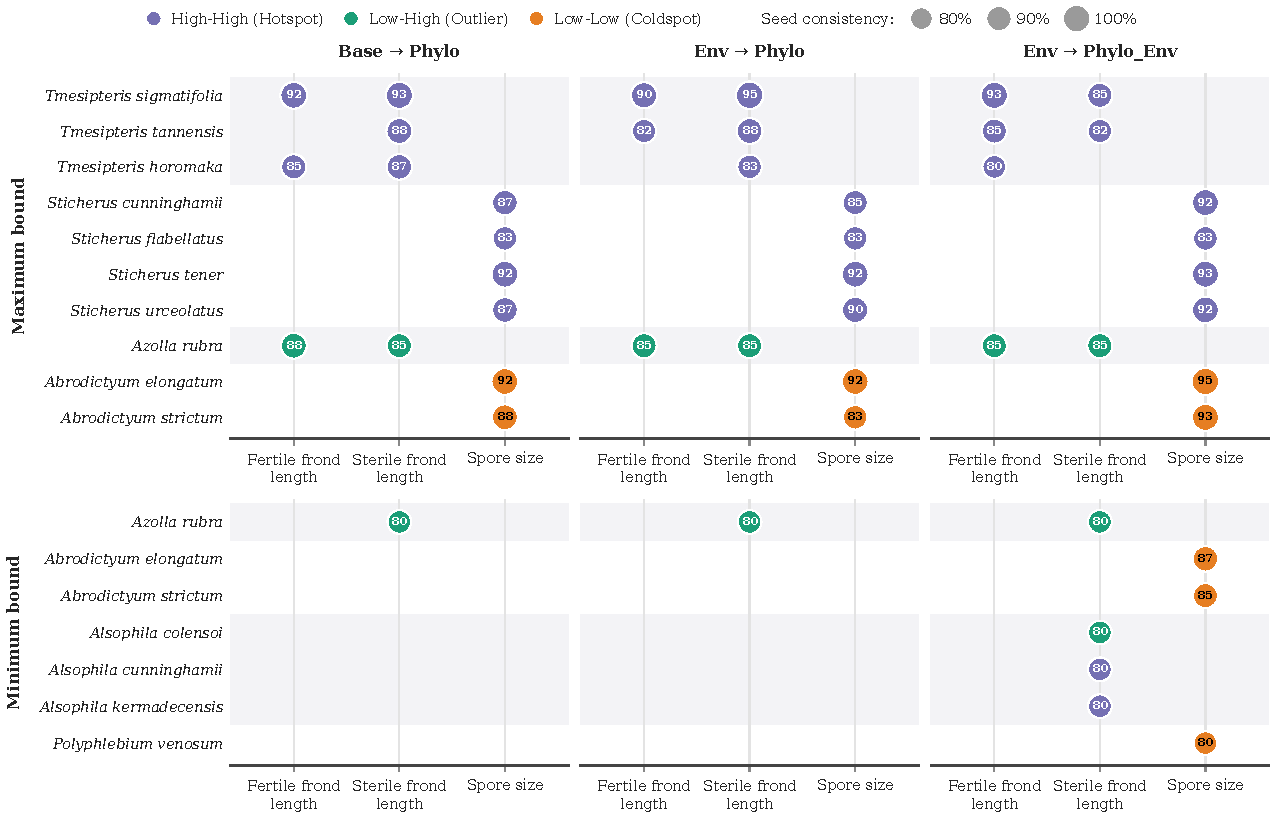
\includegraphics[width=\linewidth]{lipa_80pct_consistency_overview.pdf}
    \caption{Local Moran's I analyses showing the set of species and traits for which changes in imputation error were consistently phylogenetically structured in $\geq80\%$ of imputation seeds. Hotspots (in purple) indicate species in phylogenetic regions for which the added information produced substantial predictive gains. Coldspots (in orange) indicate species in phylogenetic regions for which the added information produced poor or negligible error reduction alongside phylogenetic neighbours of similar performance. Low--High Outliers (in green) indicate isolated species for which the added information produced sharply higher (or lower) prediction errors compared to that of their close evolutionary relatives.}
    \label{fig:moransI}
\end{figure}

For maximum sterile frond length, \textit{Tmesipteris sigmatifolia} consistently formed a hotspot in all three relevant model transitions (Figure~\ref{fig:moransI}). In addition, \textit{T.~horomaka} was a hotspot in the Base $\rightarrow$ Phylo comparison (87\%) and in the Env $\rightarrow$ Phylo comparison (83\%), indicating that phylogenetically informed models produced locally similar positive error changes across multiple \textit{Tmesipteris} species. By contrast, \textit{Azolla rubra} repeatedly occurred as a Low--High outlier for maximum and minimum sterile frond length. It was identified as an outlier in 85\% of seeds in the Base $\rightarrow$ Phylo transition, 85\% in the Env $\rightarrow$ Phylo transition, and 85\% in the Env $\rightarrow$ Phylo\_Env transition. Thus, across all maximum sterile-frond comparisons involving phylogenetic information, \textit{A.~rubra} consistently differed from the positive response of its local phylogenetic neighbourhood. The Env $\rightarrow$ Phylo\_Env transition additionally identified a structured pattern among tree ferns. \textit{Alsophila cunninghamii} and \textit{A.~kermadecensis} were hotspots for minimum sterile frond length, each in 80\% of seeds. In contrast, \textit{Alsophila colensoi} was a Low--High outlier in 80\% of seeds (Figure~\ref{fig:moransI}).

Spore size displayed a strong contrast between coldspots (i.e. species exhibiting poor or negligible error reduction alongside phylogenetic neighbours of similar performance) in \textit{Abrodictyum} and hotspots in \textit{Sticherus}. For maximum spore size, \textit{Abrodictyum elongatum} and \textit{A.~strictum} consistently formed coldspots. In the Base $\rightarrow$ Phylo transition, \textit{A.~elongatum} was a coldspot in 92\% of seeds and \textit{A.~strictum} in 88\%. In the Env $\rightarrow$ Phylo transition, these values were 92\% and 83\%, respectively. In the Env $\rightarrow$ Phylo\_Env transition, coldspot consistency increased to 95\% for \textit{A.~elongatum} and 93\% for \textit{A.~strictum}. In contrast, species of \textit{Sticherus} consistently formed hotspots for maximum spore size. In the Base $\rightarrow$ Phylo transition, \textit{Sticherus cunninghamii}, \textit{S.~flabellatus}, \textit{S.~tener}, and \textit{S.~urceolatus} were hotspots in 87\%, 83\%, 92\%, and 87\% of seeds, respectively. The Env $\rightarrow$ Phylo transition produced nearly identical results, with hotspot frequencies of 85\%, 83\%, 92\%, and 90\%. The Env $\rightarrow$ Phylo\_Env transition again recovered all four species as hotspots, with frequencies of 92\%, 83\%, 93\%, and 92\%, respectively. Thus, the \textit{Abrodictyum} and \textit{Sticherus} signals represent opposite but highly stable local phylogenetic patterns for maximum spore size (Figure~\ref{fig:moransI}).

Overall, the reproducible local patterns were concentrated in a limited number of genera. The most consistent hotspots were observed in \textit{Tmesipteris} for fertile and sterile frond lengths and in \textit{Sticherus} for sterile frond length and spore size. The strongest coldspots occurred in \textit{Abrodictyum} for spore size. \textit{Azolla rubra} was the most recurrent Low--High outlier, occurring repeatedly for fertile and sterile frond lengths across comparisons involving phylogenetic information. At minimum sterile frond length, the combined phylogenetic-plus-environmental model additionally differentiated among \textit{Alsophila} species, identifying \textit{A.~cunninghamii} and \textit{A.~kermadecensis} as hotspots and \textit{A.~colensoi} as a Low--High outlier. These results showed that phylogenetically structured changes in imputation performance were concentrated in a small subset of traits and lineages, with maximum frond dimensions and spore size displaying the strongest and most repeatable local patterns across imputation seeds.

Model performance varied across trait quantiles. In the smallest quantile, $\Delta_\mathrm{err}$ variance increased markedly across traits when either environmental or phylogenetic information was added to the model. For higher trait quantiles,  $\Delta_\mathrm{err}$ showed considerable fluctuations, yielding consistent prediction improvement across models only for the larger trait class (Figure~\ref{fig:quantone}, Figure~\ref{fig:quanthree}). Overall, these results indicate that small traits posed a general challenge across the phylogeny.

\section{Discussion}

Our results show that predictive information on fern morphology is unevenly distributed among traits, taxa, and information sources. Phylogenetic information provided the largest and most consistent reduction in imputation error, particularly for frond dimensions, whereas broad-scale environmental predictors made smaller and more target-dependent contributions. The analyses further identified where these predictive gains occurred across the phylogeny and whether they were locally structured among related species. Thus, the framework not only compared overall imputation performance, but also revealed the traits, lineages, and species for which phylogenetic and environmental information improved or constrained prediction.

Across the benchmark analyses, \awesomeModel{} was the most consistently performing method across the trait matrix. It ranked first or second for 11 of the 12 output variables and achieved the lowest NRMSE-IQR for five. Other methods performed particularly well for narrower subsets of traits: MICE performed best for minimum stipe dimensions, whereas Rphylopars performed best for maximum fertile and sterile frond length. However, \awesomeModel{} maintained comparatively stable performance across frond, stipe, and spore traits. The model therefore provides a robust general-purpose imputation approach for this heterogeneous trait matrix, although specialised methods may remain preferable for individual targets. Altitudinal range and maximum spore size were exceptions, being reconstructed as accurately, or more accurately, by simple aggregation approaches. Their relatively large errors across methods suggest that the available predictors contained limited exploitable information for these outputs. This does not imply that these traits lack biological structure, but rather that their relevant structure was not fully captured by the phylogenetic, environmental, and trait information available to the evaluated models.

The ablation analyses identified phylogenetic information as the dominant source of incremental predictive signal. Across all trait–variable slices, the median NRMSE-IQR was 4.591 for the baseline model, 4.595 after adding environmental information, 4.512 after adding phylogenetic information, and 4.511 when both information sources were included. Thus, phylogenetic information produced the clearest aggregate reduction in error, whereas environmental predictors produced no statistically significant global improvement either alone or in addition to phylogeny. Trait-specific analyses nevertheless showed that environmental predictors contributed to selected outputs, particularly frond and stipe dimensions. This pattern indicates that environmental information was not absent from the model, but that its predictive contribution was more localised, weaker on average, and partly redundant with information already represented by phylogeny and observed traits.

Attribution analysis supported this interpretation. Soil pH had the largest feature-level environmental attribution, particularly for minimum sterile stipe length, while climatic variables collectively contributed most of the total environmental attribution because they represented the largest predictor domain. These attributions describe how the trained model used the available inputs, but they do not establish that soil pH or climate directly caused the corresponding morphological variation. Nevertheless, they demonstrate that environmental information influenced particular predictions even when it yielded only limited aggregate improvement in the ablation analysis. Together, the benchmark, ablation, and attribution results establish a hierarchy of predictive information: phylogeny carried the most broadly transferable signal in this dataset, whereas environmental variables refined prediction for selected trait dimensions. The strong contribution of phylogenetic information is consistent with the ability of relatedness to capture shared ancestry, developmental constraints, correlated trait evolution, conserved ecological associations, or conserved selection (Laughlin et al., 2023; Westoby et al., 2007). However, predictive utility should not be interpreted as evidence for a single evolutionary mechanism. A phylogeny can improve trait prediction because closely related species resemble one another for several possible reasons, and the present analyses do not distinguish among these alternatives. Rather, they identify where phylogenetic relatedness provides useful predictive information and where it does not.

Local Moran’s I analyses for spore size identified a consistent contrast between the filmy-fern genera \textit{Abrodictyum} and \textit{Polyphlebium}, which repeatedly formed phylogenetic coldspots, and \textit{Sticherus}, which repeatedly formed hotspots. belong to the filmy-fern family Hymenophyllaceae, characterised by exceptionally thin laminae, often only one cell layer thick outside the veins, and by strong physiological dependence on humid conditions \citep{dubuisson2003rbc}. The group is associated with specialised habitats and may exhibit substantial responses to fine-scale conditions such as humidity, light and canopy structure that are unlikely to be captured by broad environmental layers \citep{dong2024formation, parra2009vertical, perrie2013hymenophyllum, proctor2012light, yu2023adaptational, wang2021effects}. These clades may therefore illustrate regions of the phylogeny where neither the available environmental predictors nor phylogenetic position provides substantial additional predictive information.

Several species of \textit{Tmesipteris} repeatedly formed hotspots for maximum fertile and/or sterile frond length when phylogenetic information was added to the model. \textit{Tmesipteris} belongs to the family Psilotaceae, a small, early-diverging and morphologically distinctive lineage within the fern clade, \citep{shen2018large}. \textit{Tmesipteris} species possesses highly specialised, pendulous leaves or flattened scale-like frond structures relatively conserved across species \citep{fernandez2026phylogenomic, wei2025resolving}. This is consistent with a situation in which their frond- or shoot-length traits are relatively coherent within the lineage and are insufficiently described by the non-phylogenetic predictors alone. Phylogenetic information may therefore act as a useful constraint, preventing predictions from drifting toward values typical of more distantly related terrestrial fern groups, although such underlying information may reflect shared ancestry, conserved selection, or both.

Finally, \textit{Azolla rubra} repeatedly behaved as a phylogenetic outlier for maximum fertile and sterile frond length, and for minimum sterile frond length, meaning its predictive response was consistently worse compared to that of its phylogenetic neighbours. This pattern is consistent with the highly specialised biology of \textit{Azolla}, a free-floating aquatic fern in the family Salviniaceae, with strongly reduced and modified fronds \citep{brownsey2014flora}. Its morphology and life history differ markedly from those of its close relatives, and as a result phylogenetic proximity may not provide a sufficiently direct predictor of frond size when the focal species occupies a highly distinctive functional and morphological regime. In this type of cases, precise information on niche occupancy may be more informative than phylogenetic proximity or broad ecological layers.

These results further highlight the significant advantage of this framework: not requiring phylogenetic similarity to be assigned a priori to a particular evolutionary process. Conventional phylogenetic comparative models typically impose an explicit model of trait evolution, thereby defining in advance what information is expected to be carried by phylogenetic relatedness \citep{laughlin2023plant, revell2022phylogenetic}. In contrast, our approach treated phylogenetic position as a flexible source of predictive information and asks where, across the phylogeny, this information improves trait prediction. The resulting spatial structure of prediction-error deltas therefore provides a different perspective on morphologically specialised species. A trait value that appears unusual in isolation may carry very different biological implications depending on its position in the phylogeny. Phylogenetic hotspots, such as those detected in \textit{Tmesipteris} and \textit{Sticherus}, identified lineages in which relatedness consistently contributed useful predictive information. This signal may arise through shared ancestry, phylogenetic niche conservatism, stabilising selection, developmental constraints, or other correlated processes \citep{westoby2006landplant, westoby2007generalization}. Coldspots, such as those in \textit{Abrodictyum}, identify regions where phylogeny contributed relatively little additional information for the focal trait. Outliers, such as \textit{Azolla rubra}, identify lineages whose response differs from that of their local phylogenetic neighbours. These departures are compatible with lineage-specific adaptation, evolutionary innovation, rapid trait evolution, unmeasured ecological factors, or incomplete representation of close trait analogues. The framework therefore does not identify a unique evolutionary process. Instead, it distinguishes where phylogenetic information is predictively useful, where its contribution is limited, and where relationships between phylogenetic position and trait values change abruptly across the tree. These locations provide targeted candidates for subsequent comparative, ecological, and evolutionary analyses.

The distinction between global and local analyses is illustrated by altitudinal range. Although Pagel's $\lambda$ indicated significant phylogenetic structure in some model transitions for this trait, Local Moran’s I did not identify significant individual species, hotspots, coldspots, or outliers. Pagel's $\lambda$ measures the overall correspondence between trait variation and phylogenetic covariance across the tree. A broadly distributed phylogenetic pattern can therefore produce significant global signal without being concentrated in a particular lineage.
In contrast, Local Moran’s I identifies local departures from the expected pattern, namely species or clades with unusually high, low, or contrasting changes in prediction error relative to their phylogenetic neighbours. The absence of significant local patterns for altitudinal range indicates that any phylogenetic contribution was diffuse rather than concentrated in particular species or clades. Thus, Pagel's $\lambda$ shows that phylogenetic structure can matter globally, whereas Local Moran’s I identifies where such structure is locally concentrated.

A similar distinction applies to stipe length. Trait-quantile analyses showed a marked reduction in predictive accuracy for small stipe lengths when phylogenetic or environmental information was added to the model. However, Local Moran’s I detected no significant spatial autocorrelation for fertile or sterile stipe length. This suggests that small species represent a general predictive challenge distributed across the phylogeny rather than a problem concentrated within particular evolutionary lineages. Such a pattern is consistent with widespread and potentially convergent morphological reduction across unrelated fern families.

The framework developed here could be extended to a range of questions in ecology and evolutionary biology. For example, in studies of convergent evolution, alternative evolutionary hypotheses could be treated as competing sources of predictive information, allowing researchers to ask which process best predicts the trait distributions observed across lineages. This may be particularly useful for studying repeated evolution in insular environments, where similar morphological and ecological syndromes have been documented across independent island radiations \citep{ciarle2023island, whittaker2023island}. Rather than assuming a priori that island endemism produces a particular evolutionary outcome, the framework could test whether information about island characteristics improves predictions of trait values, and whether models incorporating directional or other hypothesised evolutionary changes outperform models without such constraints. More generally, the same approach could be used to investigate whether particular environments impose stronger constraints on morphological evolution. Competing models could, for example, encode alternative allometric relationships or different responses to environmental conditions, and their relative predictive performance could be compared to determine where particular ecological contexts constrain the range of viable trait combinations. In this way, predictive modelling could provide a common framework for comparing alternative hypotheses about the processes that structure trait variation without requiring those processes themselves to be specified a priori as statistical corrections.

The scope of the dataset limits how broadly the results can be generalised. The study was limited to the fern species native to New Zealand, which provided a geographically and ecologically coherent study system but represented only a limited portion of fern diversity. The predictive performance and the phylogenetic patterns identified here may therefore depend on the lineages, environments, and trait ranges captured by this dataset. Applying the pipeline to a larger and more taxonomically and geographically diverse species set would assess how well these results transfer beyond the New Zealand flora.

The heterogeneity of the available features also limited model robustness. The model combines morphological, phylogenetic, environmental, and categorical information, but these inputs differed in their variability and in the strength of their association with each trait. The results showed that predictive accuracy varied among traits and that small trait values posed a general challenge across the phylogeny. Consequently, the framework should be interpreted as a target-dependent imputation method: its aggregate performance does not guarantee equally reliable predictions for every trait. Additional observations, more informative environmental descriptors, or target-specific model designs may improve predictions for the traits whose variation is weakly represented by the current feature set.

In conclusion, integrating phylogenetic, environmental, and trait information within a single predictive framework improved the reconstruction of fern morphology and revealed substantial heterogeneity in the sources of predictive signal. Phylogeny provided the most consistent gains overall, and Local Moran’s I further demonstrated that these gains were concentrated in particular lineages. This combination of predictive benchmarking, ablation, attribution, and local phylogenetic analysis can provide a general framework for using imputation not only to fill missing trait values, but also to investigate phylogenetic structuring and identify where biological information is structured, transferable, and limited across the tree of life.

%% The Appendices part is started with the command \appendix;
%% appendix sections are then done as normal sections
\appendix

\section{Data characterization}
\label{app:data-characterisation}

The recorded trait ranges varied across species. Figure~\ref{fig:trait-distributions} shows the minimum and maximum values for fertile and sterile fronds, fertile and sterile stipes, and spore size. It also shows the recorded elevation limits. Values are centred on each feature's median and scaled by its interquartile range, so the horizontal axis describes variation within a feature rather than differences in physical units. The figures have been limited to the $90^\mathrm{th}$ percentile to better visualize each distribution. Notably, the minimum values for Alt had a significant number of outliers in the right tail, which have been hidden from the visualization.

\begin{figure}[ht]
    \centering
    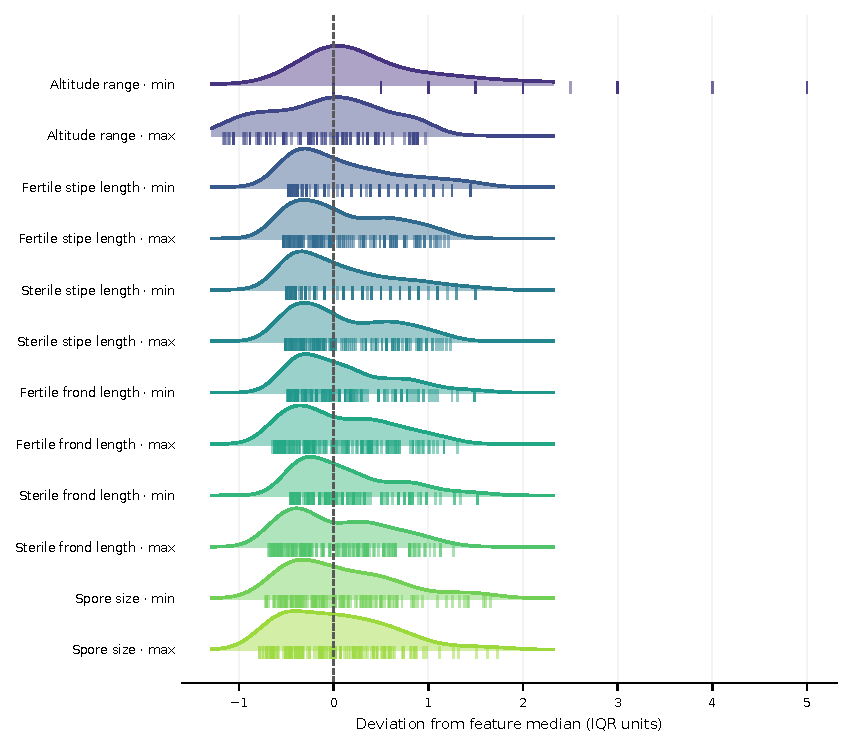
\includegraphics[width=\linewidth]{00_trait_distributions.pdf}
    \caption{Distributions of recorded trait limits and elevation limits across species. Each feature is centred on its median and expressed in interquartile-range units; ticks mark individual observations.}
    \label{fig:trait-distributions}
\end{figure}

The phylogeny (Figure~\ref{fig:phylogeny}) shows the relationships used to construct the species representations. Species are arranged on a circular tree and concentric rings report, for each species, the first two principal components (PC1, PC2) of its embedding. The rings show how the embedding coordinates vary across the phylogeny, for instance whether they are shared within clades or change between them. The embedding axes are principal components, so their signs are arbitrary, and only relative variation is informative. This plot describes the phylogenetic inputs and the structure of the extracted embeddings; it does not establish that the embeddings separate species by trait value.

\begin{figure}[ht]
    \centering
    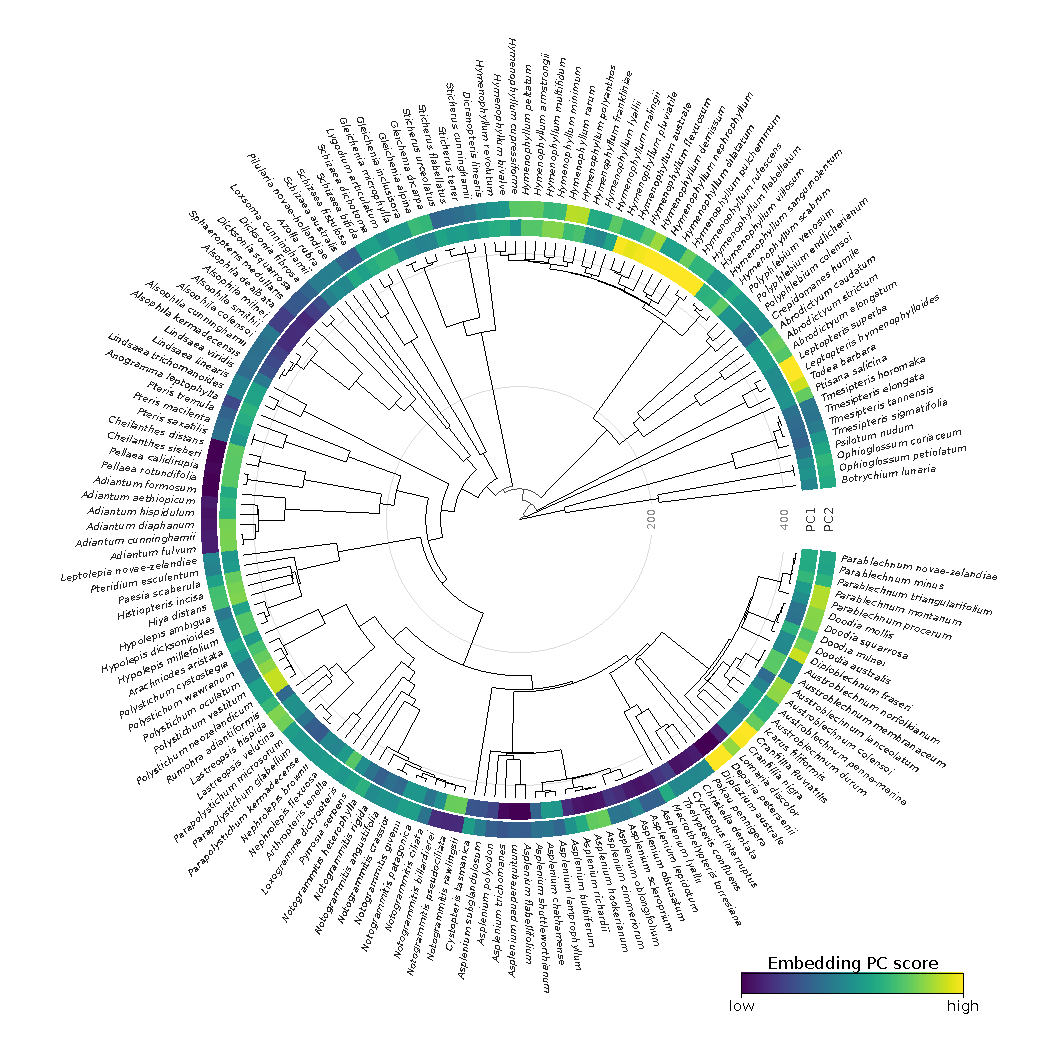
\includegraphics[width=\linewidth]{00_phylogeny_figure.pdf}
    \caption{Phylogeny of the species used in the analysis. Concentric grey circles mark branch-length distance from the root. The two outer rings show each species' embedding PC1 and PC2.}
    \label{fig:phylogeny}
\end{figure}

Environmental features varied across species and seasons (Figure~\ref{fig:environmental-features}). Solar radiation is higher in the austral summer and lower in winter (Figure~\ref{fig:solar-radiation}). Water vapour pressure follows a similar seasonal pattern, although its monthly distributions overlap (Figure~\ref{fig:vapour-pressure}). The other climate features and the soil variables differ in shape and spread after feature-wise scaling (Figures~\ref{fig:climate-features} and~\ref{fig:soil-features}).

\begin{figure}[ht]
    \centering
    \begin{subfigure}[t]{0.48\linewidth}
        \centering
        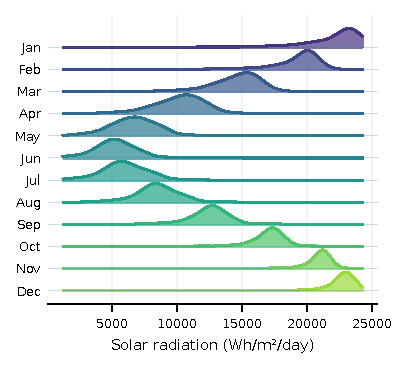
\includegraphics[width=\linewidth]{00_solar_radiation_ridgeline.pdf}
        \caption{Monthly solar radiation.}
        \label{fig:solar-radiation}
    \end{subfigure}\hfill
    \begin{subfigure}[t]{0.48\linewidth}
        \centering
        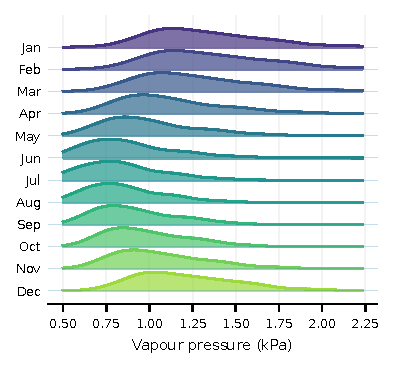
\includegraphics[width=\linewidth]{00_vapour_pressure_ridgeline.pdf}
        \caption{Monthly water vapour pressure.}
        \label{fig:vapour-pressure}
    \end{subfigure}
    \medskip
    \begin{subfigure}[b]{0.5\linewidth}
        \centering
        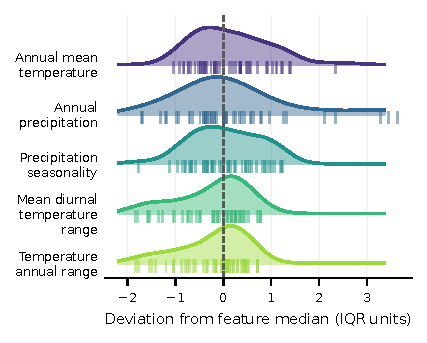
\includegraphics[width=\linewidth]{00_climate_features_distribution.pdf}
        \caption{Other climate features.}
        \label{fig:climate-features}
    \end{subfigure}\hfill
    \begin{subfigure}[b]{.5\linewidth}
        \centering
        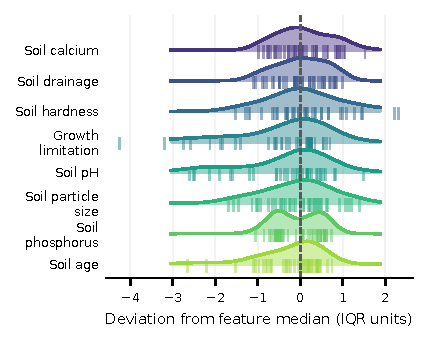
\includegraphics[width=\linewidth]{00_soil_features_distribution.pdf}
        \caption{Soil variables.}
        \label{fig:soil-features}
    \end{subfigure}

    \caption{Environmental features used in the analysis. The upper panels show monthly distributions of solar radiation in \(\mathrm{Wh\,m^{-2}\,day^{-1}}\) and water vapour pressure in \(\mathrm{kPa}\). The lower panels show feature distributions centred on their medians and scaled by their interquartile ranges; ticks mark individual observations.}
    \label{fig:environmental-features}
\end{figure}

\subsection{Environmental feature domains}
\label{app:features-domains}

The environmental input contains 45 features assigned to five domains (Table~\ref{tab:environmental-domains}). Monthly variables and position encodings are grouped in the table; each month or encoding remains a separate model input. The two ecological rasters retain the Soil domain assigned in the feature mapping.

\begin{table}[ht]
\centering
\small
\begin{tabularx}{\linewidth}{@{}Xl@{}}
\toprule
\textbf{Environmental feature} & \textbf{Domain} \\
\midrule
Solar radiation (January--December) & Climate \\
Water vapour pressure (January--December) & Climate \\
Annual mean temperature; mean diurnal and annual temperature ranges & Climate \\
Annual precipitation; precipitation seasonality & Climate \\
Elevation above sea level & Elevation \\
Position encodings (four components) & Position \\
Soil age, phosphorus, particle size, pH, growth limitation, hardness, drainage, and calcium & Soil \\
Ecological rasters (two components) & Soil \\
\bottomrule
\end{tabularx}
\caption{Environmental inputs grouped by their assigned feature domain. Parenthetical counts denote separate input features.}
\label{tab:environmental-domains}
\end{table}

\clearpage

\section{Model hyperparameters}
\label{app:hyperparameters}

Table~\ref{tab:hyperparameters} summarises the default model and data-processing settings in the implementation. Values changed by command-line arguments or experimental sweeps should be reported separately.

\begin{table}[ht]
\centering
\small
\begin{tabularx}{\linewidth}{@{}p{0.31\linewidth}p{0.17\linewidth}X@{}}
\toprule
Hyperparameter & Value & Description \\
\midrule
\multicolumn{3}{@{}l}{\emph{Model and training}} \\
Graph convolution & GATv2Conv & Attention layer in the spatial and species graph networks. \\
Layers; hidden width & 2; 150 & Layers per graph network; hidden channels. \\
Attention heads & 4 & Heads in each graph attention layer; outputs are averaged. \\
Dropout & 0.4 & Dropout passed to the graph attention layers. \\
Optimizer; learning rate & Adam; \(10^{-3}\) & Parameter update rule and initial learning rate. \\
Epoch limit; schedule & 1,000; cosine & Maximum training epochs and cosine learning-rate annealing. \\
Reconstruction loss & Huber & Deterministic loss, averaged across observed traits. \\
Training mask; visible weight & 0.15; 0.2 & Fraction of observed trait entries masked per epoch; relative loss weight on visible entries. \\
Validation mask & 0.15 & Fraction of observed training entries held out for checkpoint selection. \\
Gradient clipping & 1.0 & Maximum gradient norm. \\
\midrule
\multicolumn{3}{@{}l}{\emph{Dataset, graphs, and normalisation}} \\

Phylogenetic embedding & 16; 30; 200 & Node2Vec dimensions, walk length, and walks per node; context window is 10. \\

Spatial graph & 50; 6 & Spatial clusters and nearest neighbours per cluster. \\
Trait normalisation & Yeo--Johnson, then \(z\) & Applied separately to minimum and maximum values. \\
Other normalisation & \(z\); sine--cosine & Standardisation of environmental, categorical, and edge features; angular encoding of coordinates. Phylogenetic embeddings are left unscaled. \\
\bottomrule

\end{tabularx}

\caption{Model and data pipeline hyperparameters. Normalisation statistics are fitted on the outer-training species in each fold.}
\label{tab:hyperparameters}
\end{table}

\clearpage

\section{Supplementary figures}
\label{app1}

\setcounter{figure}{0}
\renewcommand{\thefigure}{S\arabic{figure}}

\begin{figure}
    \centering
    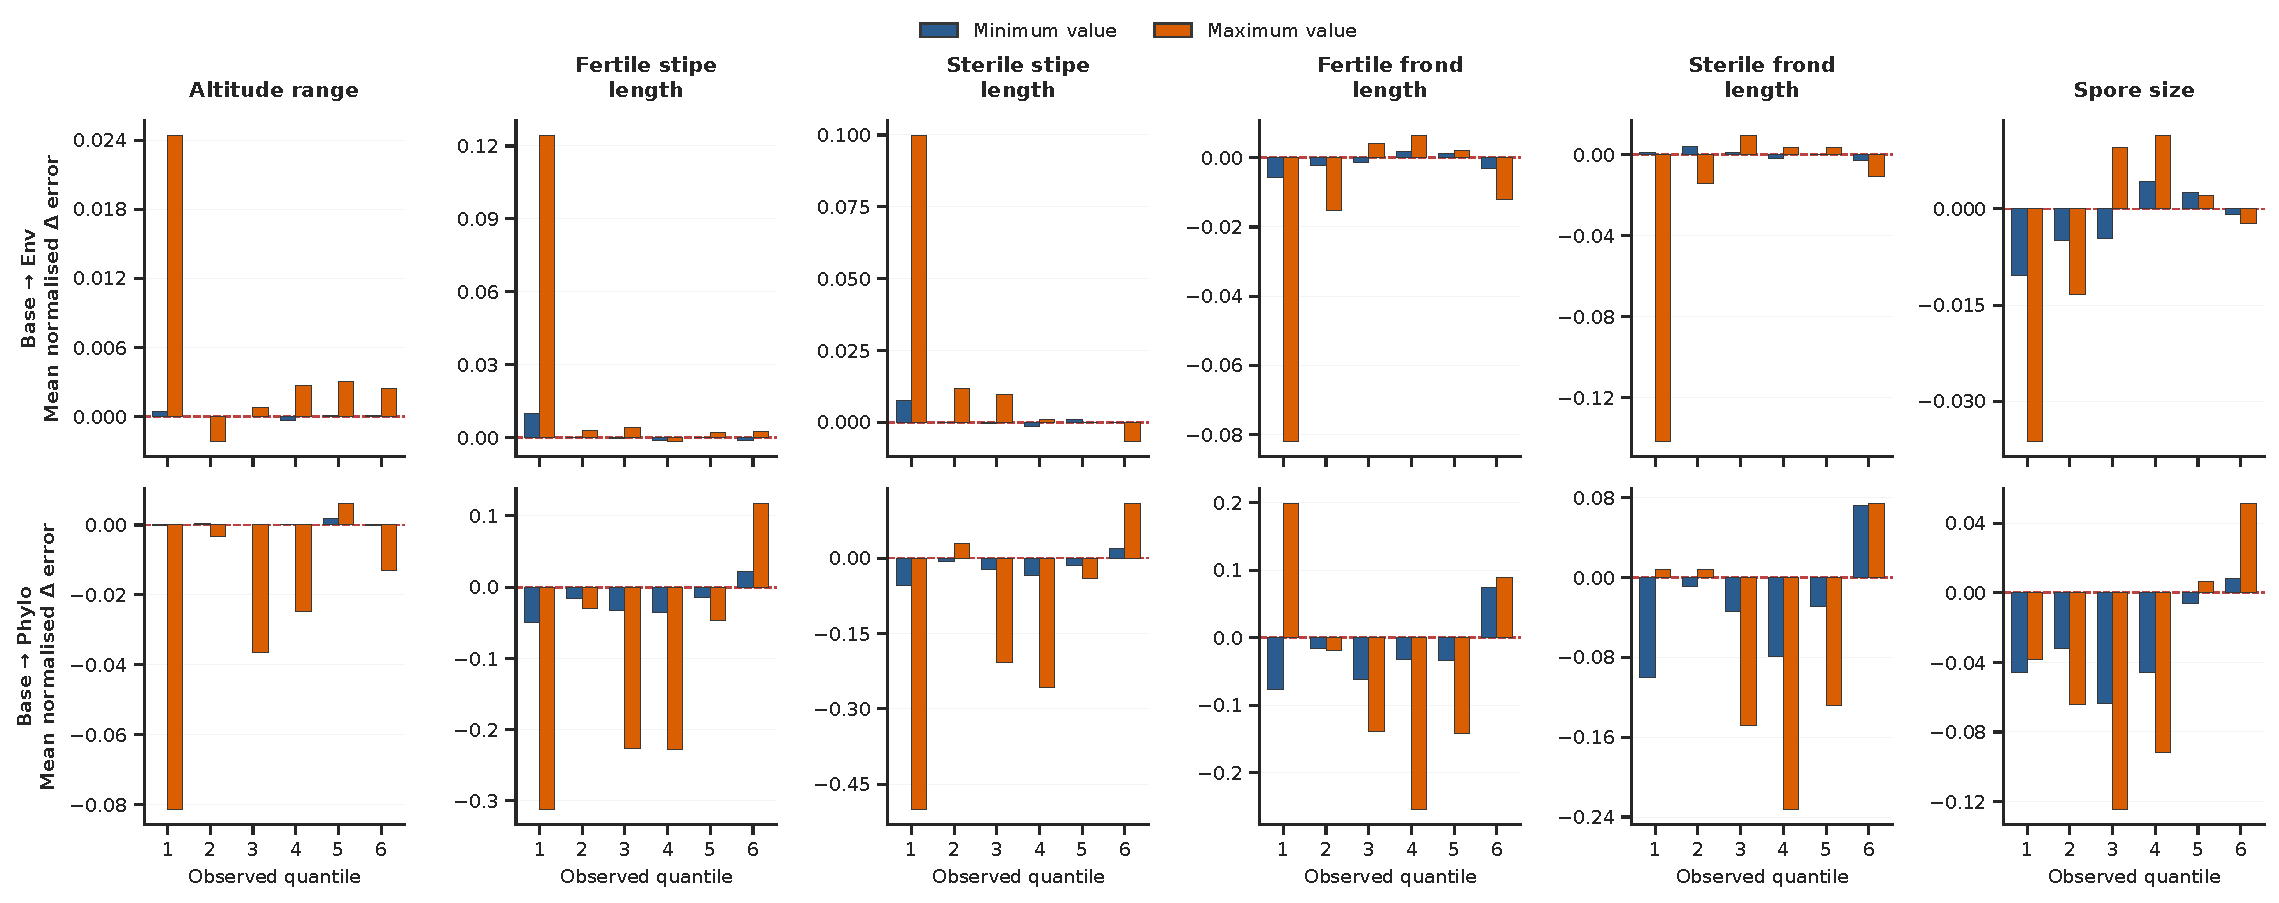
\includegraphics[width=1\linewidth]{trait_quantiles_base_transitions.pdf}
    \caption{Mean proportional change in imputation error across observed trait-value quantiles for the Base $\rightarrow$ Phylo and Base $\rightarrow$ Env models. Bars show the mean difference in normalised absolute error between the Base and Env models for each trait, separately for minimum (in blue) and maximum (in orange) trait values. Quantiles were defined from observed values within each trait, with Quantile 1 representing the smallest values and Quantile 6 the largest. Positive values indicate lower error in the Env model relative to the Base model, whereas negative values indicate increased error after adding environmental predictors.}
    \label{fig:quantone}
\end{figure}

\begin{figure}
    \centering
    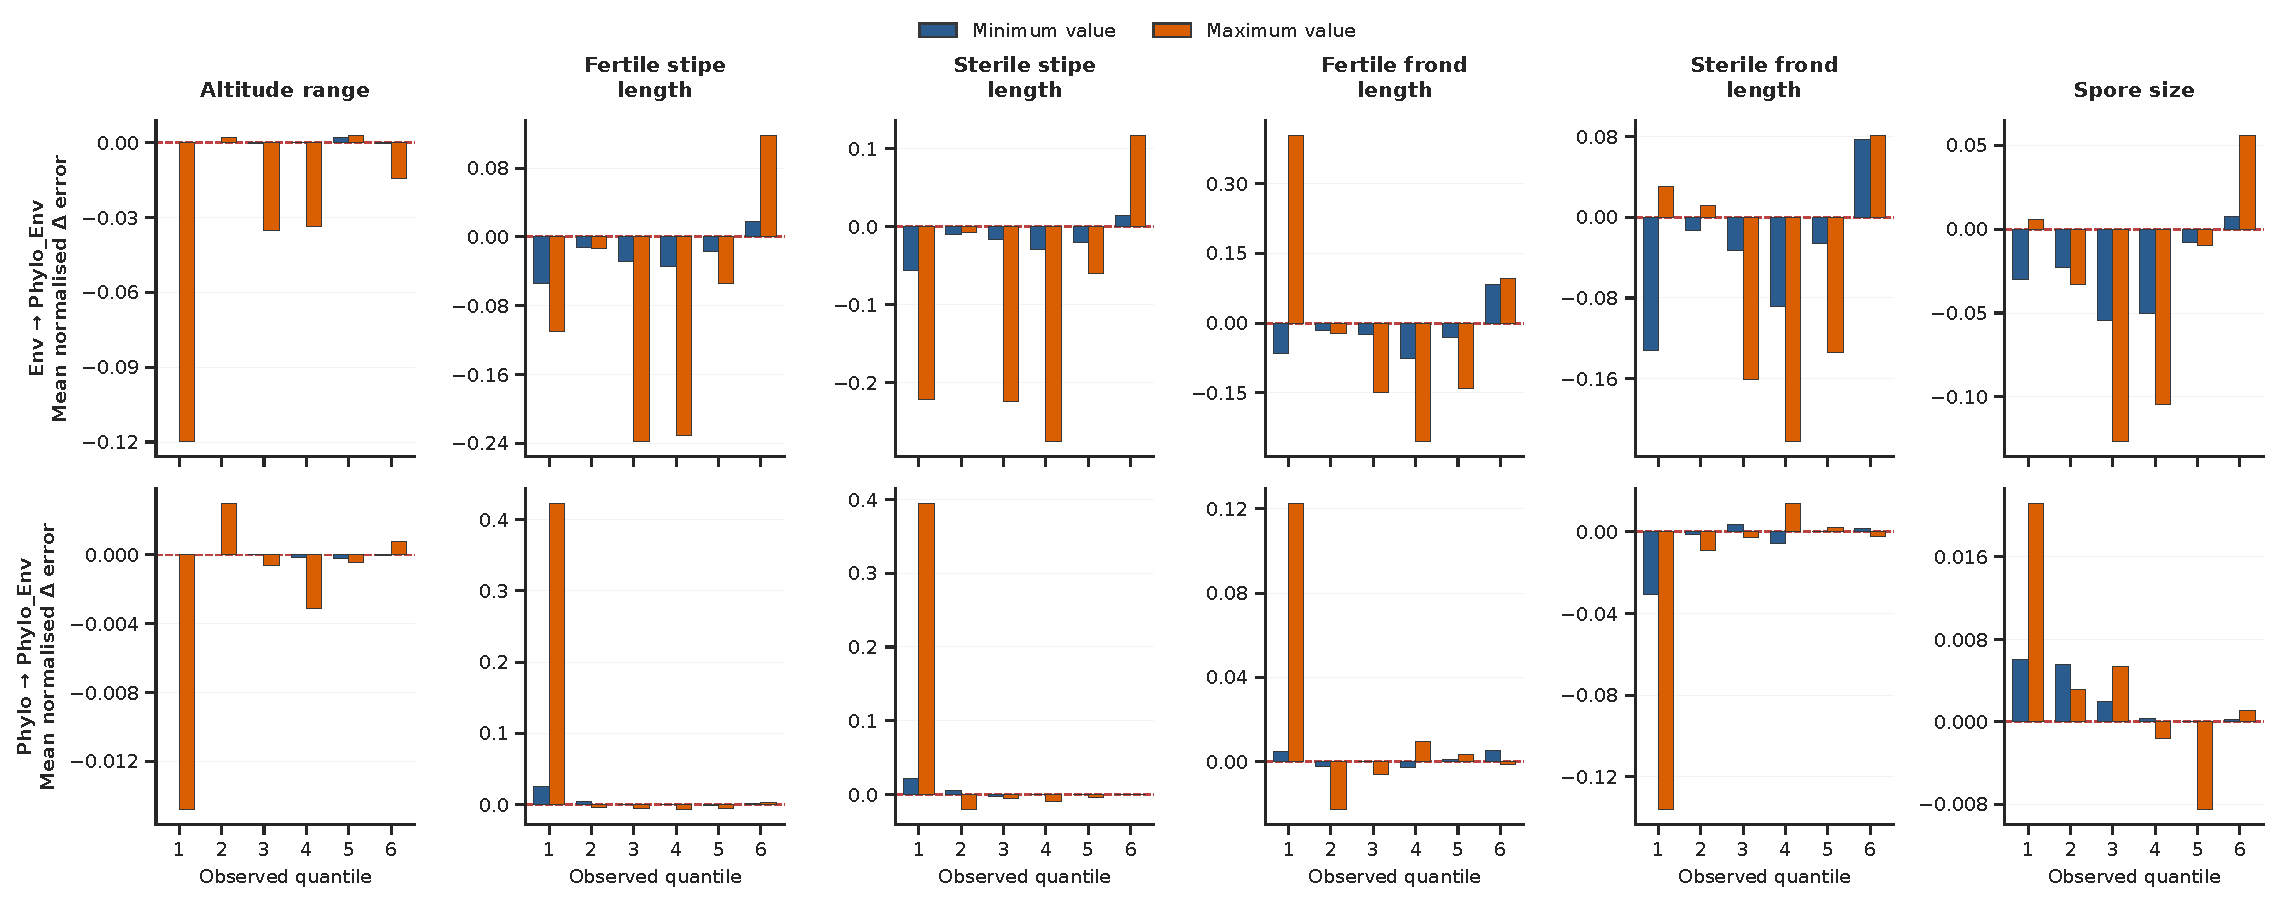
\includegraphics[width=1\linewidth]{trait_quantiles_phyloenv_transitions.pdf}
    \caption{Mean proportional change in imputation error across observed trait-value quantiles for the Env $\rightarrow$ PhyloEnv and Phylo $\rightarrow$ PhyloEnv models. Bars show the mean difference in normalised absolute error between the Base and Env models for each trait, separately for minimum (in blue) and maximum (in orange) trait values. Quantiles were defined from observed values within each trait, with Quantile 1 representing the smallest values and Quantile 6 the largest. Positive values indicate lower error in the Env model relative to the Base model, whereas negative values indicate increased error after adding environmental predictors.}
    \label{fig:quanthree}
\end{figure}

\begin{figure}
    \centering
    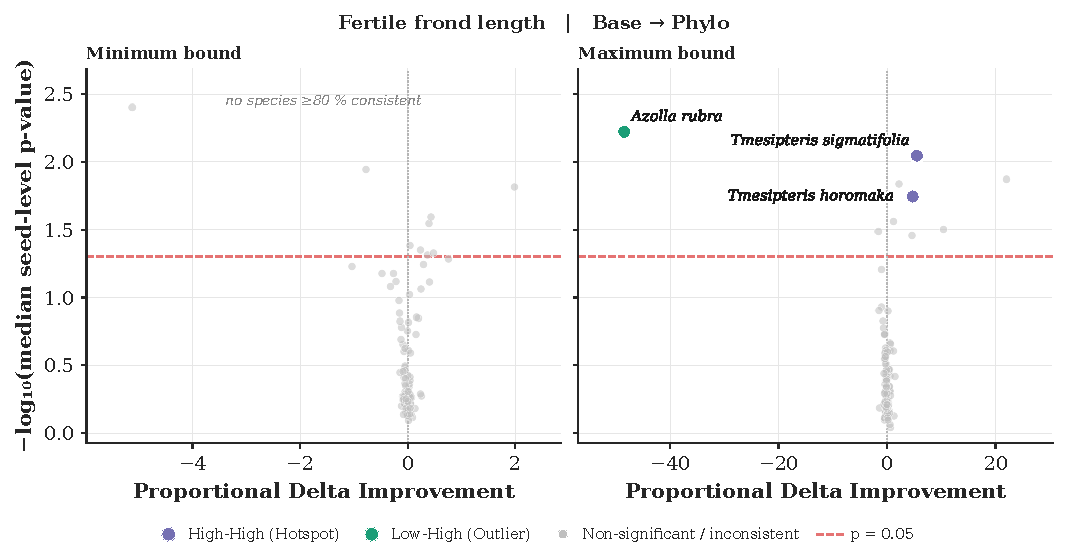
\includegraphics[width=1\linewidth]{lipa_80pct_Base_Phylo__FertileFrond.pdf}
    \caption{Consistent local phylogenetic patterns in prediction improvement for minimum and maximum fertile frond length. Points represent species assigned to the same significant Moran category in at least 80\% of imputation seeds for the Base-to-Phylogeny model transition. The x-axis shows mean proportional improvement in imputation error across seeds, with positive values indicating lower error after adding phylogenetic information. The y-axis shows the median seed-level Moran significance. The dashed line denotes p=0.05.}
    \label{fig:Moran1}
\end{figure}

\begin{figure}
    \centering
    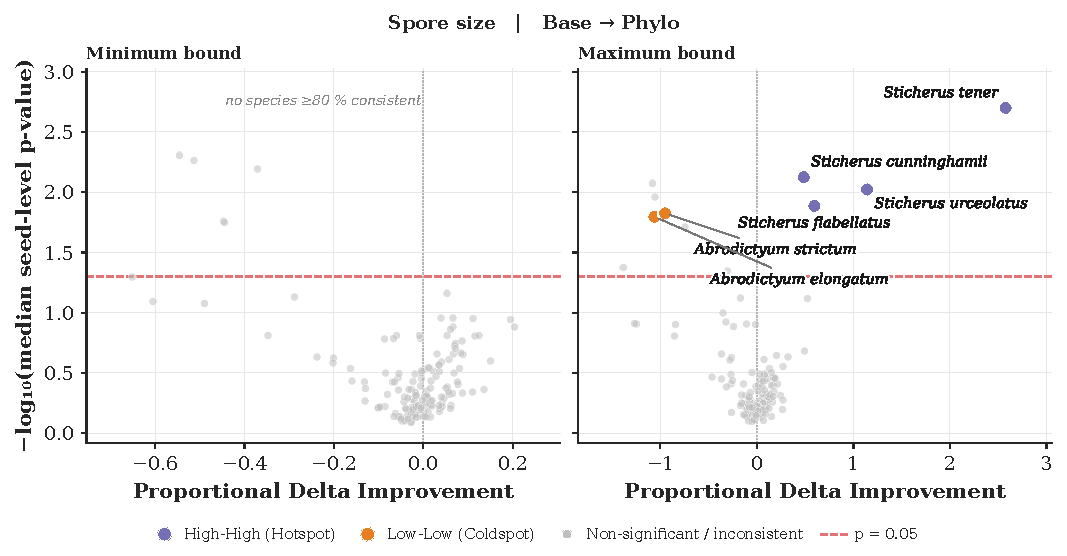
\includegraphics[width=1\linewidth]{lipa_80pct_Base_Phylo__Spore.pdf}
    \caption{Consistent local phylogenetic patterns in prediction improvement for minimum and maximum spore size. Points represent species assigned to the same significant Moran category in at least 80\% of imputation seeds for the Base-to-Phylogeny model transition. The x-axis shows mean proportional improvement in imputation error across seeds, with positive values indicating lower error after adding phylogenetic information. The y-axis shows the median seed-level Moran significance. The dashed line denotes p=0.05.}
    \label{fig:Moran2}
\end{figure}

\begin{figure}
    \centering
    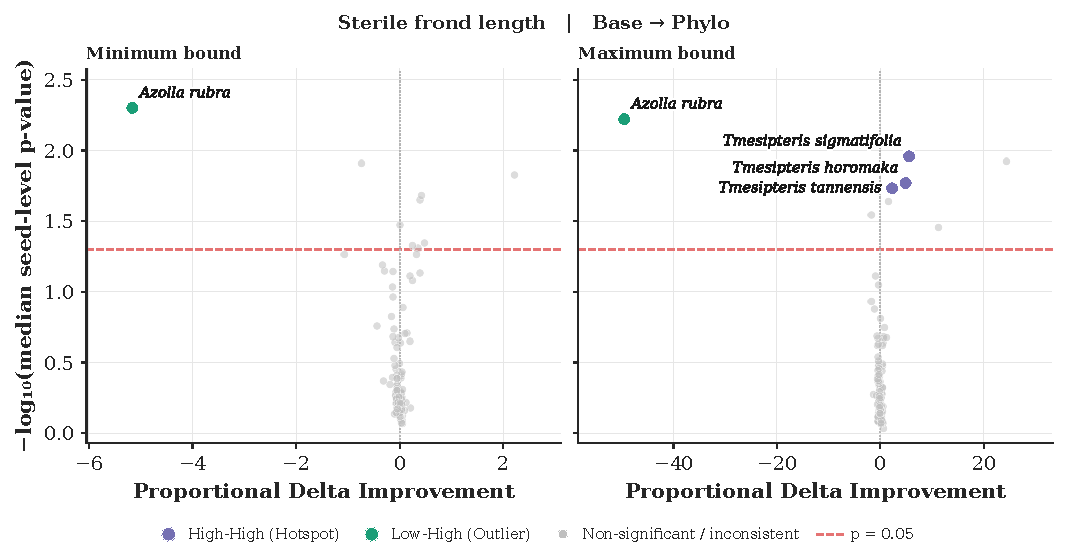
\includegraphics[width=1\linewidth]{lipa_80pct_Base_Phylo__SterileFrond.pdf}
    \caption{Consistent local phylogenetic patterns in prediction improvement for minimum and maximum sterile frond length. Points represent species assigned to the same significant Moran category in at least 80\% of imputation seeds for the Base-to-Phylogeny model transition. The x-axis shows mean proportional improvement in imputation error across seeds, with positive values indicating lower error after adding phylogenetic information. The y-axis shows the median seed-level Moran significance. The dashed line denotes p=0.05.}
    \label{fig:Moran3}
\end{figure}

\begin{figure}
    \centering
    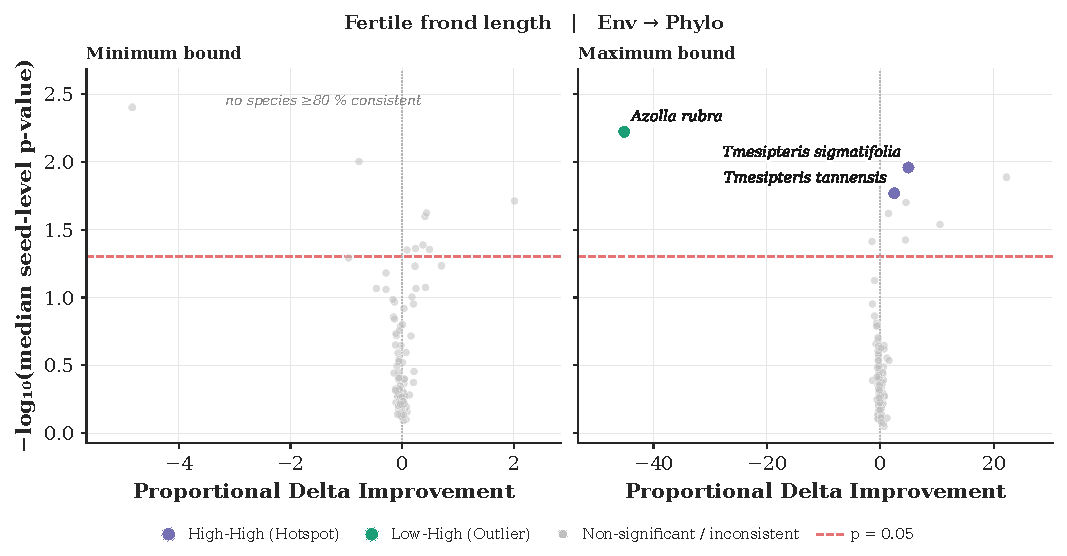
\includegraphics[width=1\linewidth]{lipa_80pct_Env_Phylo__FertileFrond.pdf}
    \caption{Consistent local phylogenetic patterns in prediction improvement for minimum and maximum fertile frond length. Points represent species assigned to the same significant Moran category in at least 80\% of imputation seeds for the Env-to-Phylogeny model transition. The x-axis shows mean proportional improvement in imputation error across seeds, with positive values indicating lower error after adding phylogenetic information. The y-axis shows the median seed-level Moran significance. The dashed line denotes p=0.05.}
    \label{fig:Moran4}
\end{figure}

\begin{figure}
    \centering
    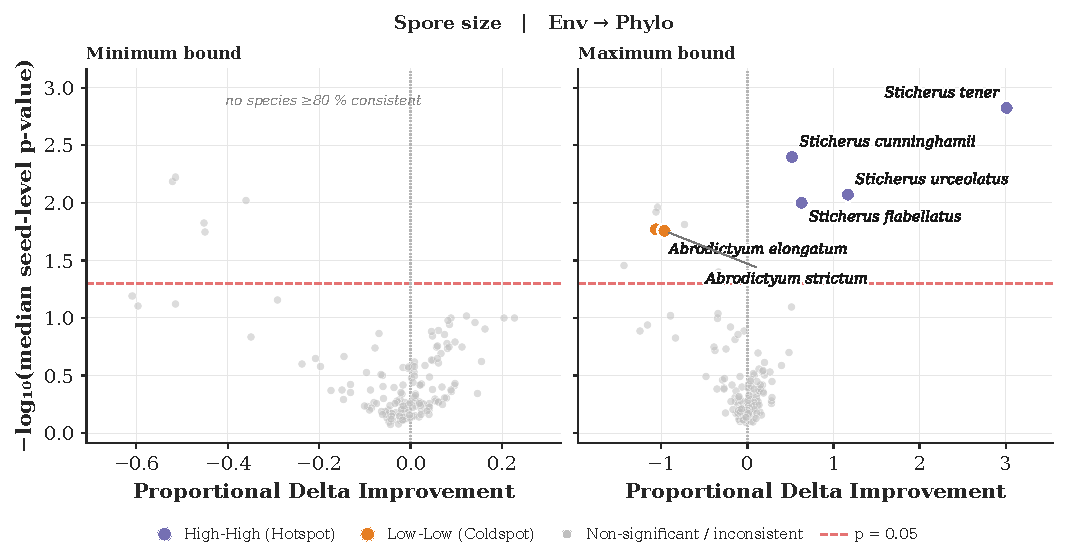
\includegraphics[width=1\linewidth]{lipa_80pct_Env_Phylo__Spore.pdf}
    \caption{Consistent local phylogenetic patterns in prediction improvement for minimum and maximum spore size. Points represent species assigned to the same significant Moran category in at least 80\% of imputation seeds for the Env-to-Phylogeny model transition. The x-axis shows mean proportional improvement in imputation error across seeds, with positive values indicating lower error after adding phylogenetic information. The y-axis shows the median seed-level Moran significance. The dashed line denotes p=0.05.}
    \label{fig:Moran5}
\end{figure}

\begin{figure}
    \centering
    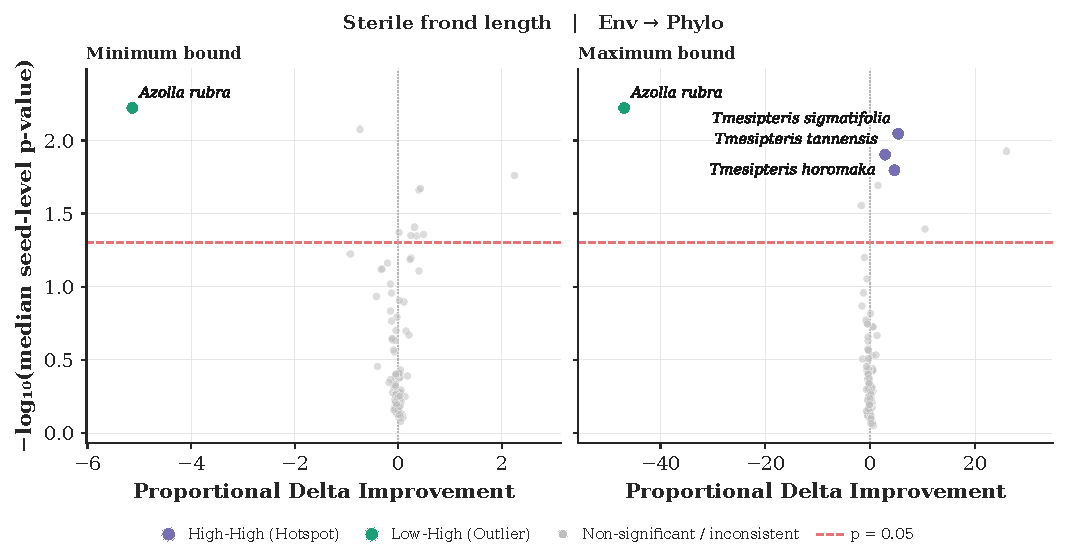
\includegraphics[width=1\linewidth]{lipa_80pct_Env_Phylo__SterileFrond.pdf}
    \caption{Consistent local phylogenetic patterns in prediction improvement for minimum and maximum sterile frond length. Points represent species assigned to the same significant Moran category in at least 80\% of imputation seeds for the Env-to-Phylogeny model transition. The x-axis shows mean proportional improvement in imputation error across seeds, with positive values indicating lower error after adding phylogenetic information. The y-axis shows the median seed-level Moran significance. The dashed line denotes p=0.05.}
    \label{fig:Moran6_1}
\end{figure}

\begin{figure}
    \centering
    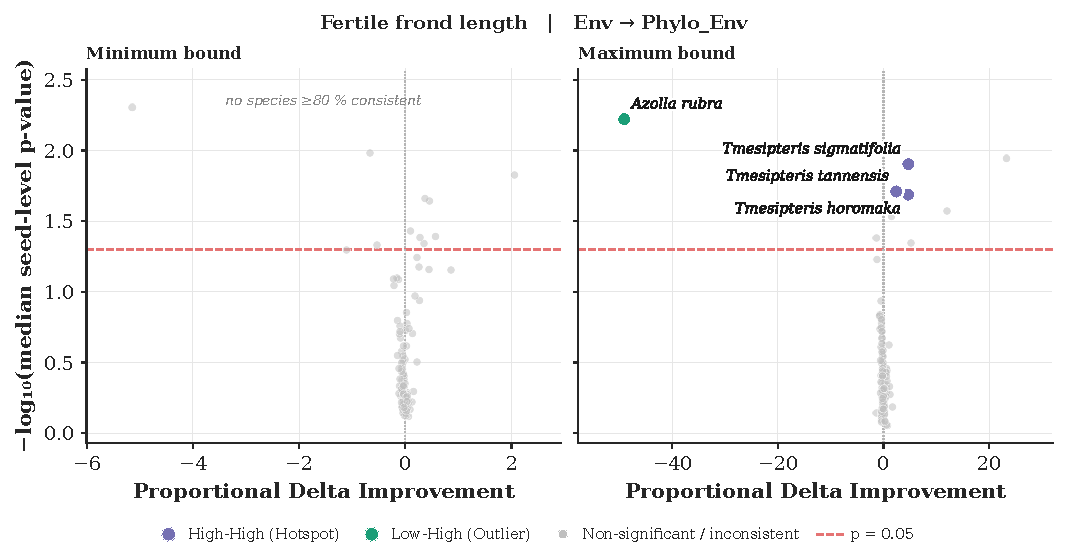
\includegraphics[width=1\linewidth]{lipa_80pct_Env_Phylo_Env__FertileFrond.pdf}
    \caption{Consistent local phylogenetic patterns in prediction improvement for minimum and maximum fertile frond length. Points represent species assigned to the same significant Moran category in at least 80\% of imputation seeds for the Env-to-EnvPhylogeny model transition. The x-axis shows mean proportional improvement in imputation error across seeds, with positive values indicating lower error after adding phylogenetic information. The y-axis shows the median seed-level Moran significance. The dashed line denotes p=0.05.}
    \label{fig:Moran6_2}
\end{figure}

\begin{figure}
    \centering
    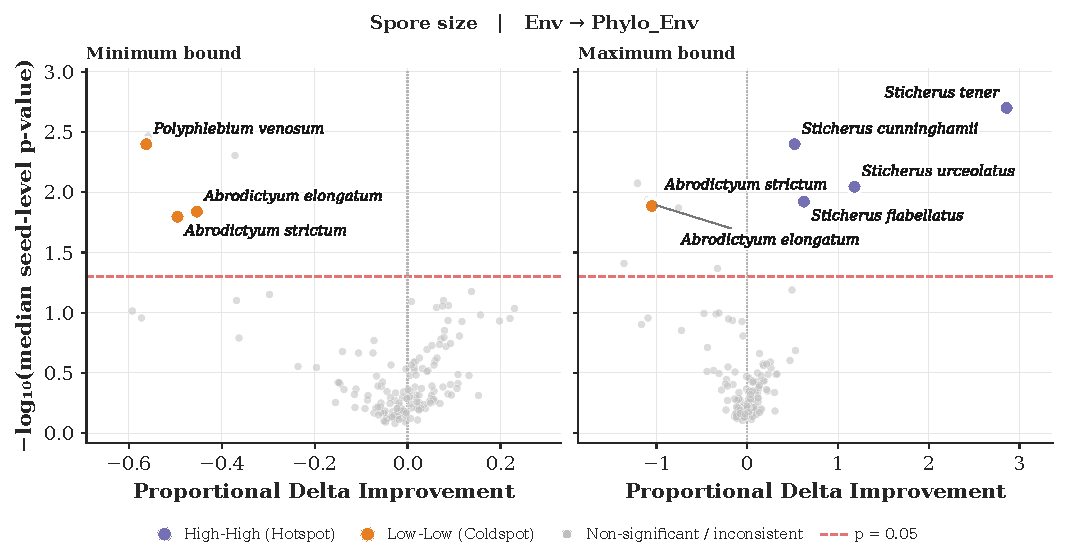
\includegraphics[width=1\linewidth]{lipa_80pct_Env_Phylo_Env__Spore.pdf}
    \caption{Consistent local phylogenetic patterns in prediction improvement for minimum and maximum spore size. Points represent species assigned to the same significant Moran category in at least 80\% of imputation seeds for the Env-to-EnvPhylogeny model transition. The x-axis shows mean proportional improvement in imputation error across seeds, with positive values indicating lower error after adding phylogenetic information. The y-axis shows the median seed-level Moran significance. The dashed line denotes p=0.05.}
    \label{fig:Moran6_3}
\end{figure}

\begin{figure}
    \centering
    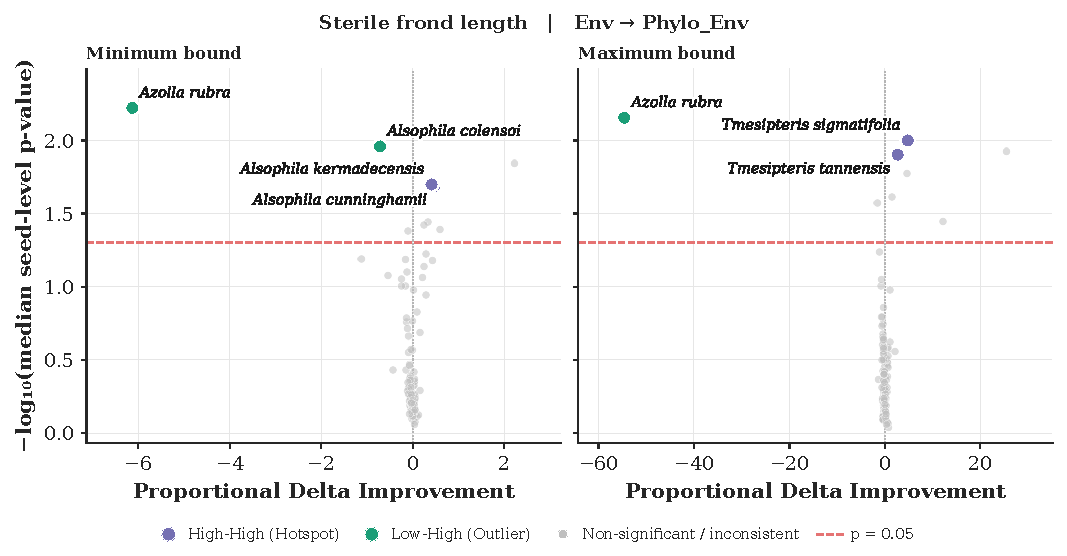
\includegraphics[width=1\linewidth]{lipa_80pct_Env_Phylo_Env__SterileFrond.pdf}
    \caption{Consistent local phylogenetic patterns in prediction improvement for minimum and maximum sterile frond length. Points represent species assigned to the same significant Moran category in at least 80\% of imputation seeds for the Env-to-EnvPhylogeny model transition. The x-axis shows mean proportional improvement in imputation error across seeds, with positive values indicating lower error after adding phylogenetic information. The y-axis shows the median seed-level Moran significance. The dashed line denotes p=0.05.}
    \label{fig:Moran6_4}
\end{figure}

\clearpage
%% For citations use: 
%%       \citet{<label>} ==> Lamport (1994)
%%       \citep{<label>} ==> (Lamport, 1994)
%%

%% If you have bib database file and want bibtex to generate the
%% bibitems, please use
%%
%\bibliographystyle{elsarticle-harv} 
%\bibliography{zotero, cas-refs}

%\input{output.bbl}

%% else use the following coding to input the bibitems directly in the
%% TeX file.

%% Refer following link for more details about bibliography and citations.
%% https://en.wikibooks.org/wiki/LaTeX/Bibliography_Management

% \begin{thebibliography}{00}
\begin{thebibliography}{69}
\expandafter\ifx\csname natexlab\endcsname\relax\def\natexlab#1{#1}\fi
\providecommand{\url}[1]{\texttt{#1}}
\providecommand{\href}[2]{#2}
\providecommand{\path}[1]{#1}
\providecommand{\DOIprefix}{doi:}
\providecommand{\ArXivprefix}{arXiv:}
\providecommand{\URLprefix}{URL: }
\providecommand{\Pubmedprefix}{pmid:}
\providecommand{\doi}[1]{\href{http://dx.doi.org/#1}{\path{#1}}}
\providecommand{\Pubmed}[1]{\href{pmid:#1}{\path{#1}}}
\providecommand{\bibinfo}[2]{#2}
\ifx\xfnm\relax \def\xfnm[#1]{\unskip,\space#1}\fi
%Type = Article
\bibitem[{Ackerly(2009)}]{ackerly2009conservatism}
\bibinfo{author}{Ackerly, D.}, \bibinfo{year}{2009}.
\newblock \bibinfo{title}{Conservatism and diversification of plant functional traits: {Evolutionary} rates versus phylogenetic signal}.
\newblock \bibinfo{journal}{Proceedings of the National Academy of Sciences} \bibinfo{volume}{106}, \bibinfo{pages}{19699--19706}.
\newblock \DOIprefix\doi{10.1073/pnas.0901635106}.
%Type = Article
\bibitem[{Adler et~al.(2014)Adler, Salguero-Gómez, Compagnoni, Hsu, Ray-Mukherjee, Mbeau-Ache and Franco}]{adler_functional_2014}
\bibinfo{author}{Adler, P.B.}, \bibinfo{author}{Salguero-Gómez, R.}, \bibinfo{author}{Compagnoni, A.}, \bibinfo{author}{Hsu, J.S.}, \bibinfo{author}{Ray-Mukherjee, J.}, \bibinfo{author}{Mbeau-Ache, C.}, \bibinfo{author}{Franco, M.}, \bibinfo{year}{2014}.
\newblock \bibinfo{title}{Functional traits explain variation in plant life history strategies}.
\newblock \bibinfo{journal}{Proceedings of the National Academy of Sciences} \bibinfo{volume}{111}, \bibinfo{pages}{740--745}.
\newblock \URLprefix \url{https://www.pnas.org/doi/full/10.1073/pnas.1315179111}, \DOIprefix\doi{10.1073/pnas.1315179111}.
%Type = Article
\bibitem[{Albassatneh et~al.(2023)Albassatneh, Dubuisson, Escudero, Fady, Ponger and Muller}]{albassatneh2023effect}
\bibinfo{author}{Albassatneh, M.C.}, \bibinfo{author}{Dubuisson, J.}, \bibinfo{author}{Escudero, M.}, \bibinfo{author}{Fady, B.}, \bibinfo{author}{Ponger, L.}, \bibinfo{author}{Muller, S.}, \bibinfo{year}{2023}.
\newblock \bibinfo{title}{Effect of environmental and spatial factors on the phylogenetic and functional diversity of the {Mediterranean} tree communities of {Europe}}.
\newblock \bibinfo{journal}{Plant Biology} \bibinfo{volume}{25}, \bibinfo{pages}{631--645}.
\newblock \DOIprefix\doi{10.1111/plb.13525}.
%Type = Article
\bibitem[{Anselin(1995)}]{anselin1995local}
\bibinfo{author}{Anselin, L.}, \bibinfo{year}{1995}.
\newblock \bibinfo{title}{Local {Indicators} of {Spatial} {Association—LISA}}.
\newblock \bibinfo{journal}{Geographical Analysis} \bibinfo{volume}{27}, \bibinfo{pages}{93--115}.
\newblock \DOIprefix\doi{10.1111/j.1538-4632.1995.tb00338.x}.
%Type = Article
\bibitem[{Bronstein et~al.(2021)Bronstein, Bruna, Cohen and Veli{\v{c}}kovi{\'c}}]{bronstein2021geometric}
\bibinfo{author}{Bronstein, M.M.}, \bibinfo{author}{Bruna, J.}, \bibinfo{author}{Cohen, T.}, \bibinfo{author}{Veli{\v{c}}kovi{\'c}, P.}, \bibinfo{year}{2021}.
\newblock \bibinfo{title}{Geometric deep learning: Grids, groups, graphs, geodesics, and gauges}.
\newblock \bibinfo{journal}{arXiv preprint arXiv:2104.13478} .
%Type = Article
\bibitem[{Brownsey and Perrie(2014)}]{brownsey2014flora}
\bibinfo{author}{Brownsey, P.}, \bibinfo{author}{Perrie, L.}, \bibinfo{year}{2014}.
\newblock \bibinfo{title}{Flora of new zealand ferns and lycophytes}.
\newblock \bibinfo{journal}{Breitwieser, I. Heenan, Wilton, AD Flora of New Zealand} .
%Type = Article
\bibitem[{Caruso et~al.(2020)Caruso, Mason and Medeiros}]{caruso2020evolution}
\bibinfo{author}{Caruso, C.M.}, \bibinfo{author}{Mason, C.M.}, \bibinfo{author}{Medeiros, J.S.}, \bibinfo{year}{2020}.
\newblock \bibinfo{title}{The {Evolution} of {Functional} {Traits} in {Plants}: {Is} the {Giant} {Still} {Sleeping}?}
\newblock \bibinfo{journal}{International Journal of Plant Sciences} \bibinfo{volume}{181}, \bibinfo{pages}{1--8}.
\newblock \DOIprefix\doi{10.1086/707141}.
%Type = Article
\bibitem[{Chamberlain et~al.(2017)Chamberlain, Ram, Barve, Mcglinn and Chamberlain}]{chamberlain2017package}
\bibinfo{author}{Chamberlain, S.}, \bibinfo{author}{Ram, K.}, \bibinfo{author}{Barve, V.}, \bibinfo{author}{Mcglinn, D.}, \bibinfo{author}{Chamberlain, M.S.}, \bibinfo{year}{2017}.
\newblock \bibinfo{title}{Package ‘rgbif’}.
\newblock \bibinfo{journal}{Interface to the Global Biodiversity Information Facility ‘API} \bibinfo{volume}{5}.
%Type = Article
\bibitem[{Ciarle(2025)}]{ciarle2025disentangling}
\bibinfo{author}{Ciarle, R.}, \bibinfo{year}{2025}.
\newblock \bibinfo{title}{Disentangling the relative roles of biased colonization and in situ evolution in driving the island syndrome in {Coprosma} {(Rubiaceae})}.
\newblock \bibinfo{journal}{Oikos} \bibinfo{volume}{2026}.
\newblock \DOIprefix\doi{10.1002/oik.11782}.
%Type = Article
\bibitem[{Ciarle and Burns(2023)}]{ciarle2023island}
\bibinfo{author}{Ciarle, R.}, \bibinfo{author}{Burns, K.C.}, \bibinfo{year}{2023}.
\newblock \bibinfo{title}{Island biogeography of birds in the {South} {West} {Pacific}: {Direct} and indirect effects of physical geography and co‐occurring vegetation}.
\newblock \bibinfo{journal}{Journal of Biogeography} \bibinfo{volume}{51}, \bibinfo{pages}{1623--1631}.
\newblock \DOIprefix\doi{10.1111/jbi.14731}.
%Type = Article
\bibitem[{Crisp and Cook(2012)}]{crisp2012phylogenetic}
\bibinfo{author}{Crisp, M.D.}, \bibinfo{author}{Cook, L.G.}, \bibinfo{year}{2012}.
\newblock \bibinfo{title}{Phylogenetic niche conservatism: what are the underlying evolutionary and ecological causes?}
\newblock \bibinfo{journal}{New Phytologist} \bibinfo{volume}{196}, \bibinfo{pages}{681--694}.
\newblock \DOIprefix\doi{10.1111/j.1469-8137.2012.04298.x}.
%Type = Article
\bibitem[{Cruz-Nicolás and Gernandt(2025)}]{cruznicolas2025combination}
\bibinfo{author}{Cruz-Nicolás, J.}, \bibinfo{author}{Gernandt, D.S.}, \bibinfo{year}{2025}.
\newblock \bibinfo{title}{A combination of stabilizing selection and random walk are associated with phylogenetic signal in hard pines}.
\newblock \bibinfo{journal}{Annals of Botany} \bibinfo{volume}{136}, \bibinfo{pages}{821--836}.
\newblock \DOIprefix\doi{10.1093/aob/mcaf147}.
%Type = Article
\bibitem[{Dong et~al.(2024)Dong, Tong, Liao, Yi, Yan and Yu}]{dong2024formation}
\bibinfo{author}{Dong, D.}, \bibinfo{author}{Tong, J.}, \bibinfo{author}{Liao, L.}, \bibinfo{author}{Yi, L.}, \bibinfo{author}{Yan, W.}, \bibinfo{author}{Yu, F.}, \bibinfo{year}{2024}.
\newblock \bibinfo{title}{Formation of single-dominant-species patches of dicranopteris dichotoma primarily influenced by understory light intensity}.
\newblock \bibinfo{journal}{Frontiers in Plant Science} \bibinfo{volume}{15}, \bibinfo{pages}{1444371}.
%Type = Article
\bibitem[{Dubuisson et~al.(2003)Dubuisson, Hennequin, Douzery, Cranfill, Smith and Pryer}]{dubuisson2003rbc}
\bibinfo{author}{Dubuisson, J.Y.}, \bibinfo{author}{Hennequin, S.}, \bibinfo{author}{Douzery, E.J.}, \bibinfo{author}{Cranfill, R.B.}, \bibinfo{author}{Smith, A.R.}, \bibinfo{author}{Pryer, K.M.}, \bibinfo{year}{2003}.
\newblock \bibinfo{title}{rbc l phylogeny of the fern genus trichomanes (hymenophyllaceae), with special reference to neotropical taxa}.
\newblock \bibinfo{journal}{International Journal of Plant Sciences} \bibinfo{volume}{164}, \bibinfo{pages}{753--761}.
%Type = Article
\bibitem[{Díaz et~al.(2016)Díaz, Kattge, Cornelissen, Wright, Lavorel, Dray, Reu, Kleyer, Wirth, Colin~Prentice, Garnier, Bönisch, Westoby, Poorter, Reich, Moles, Dickie, Gillison, Zanne, Chave, Joseph~Wright, Sheremet’ev, Jactel, Baraloto, Cerabolini, Pierce, Shipley, Kirkup, Casanoves, Joswig, Günther, Falczuk, Rüger, Mahecha and Gorné}]{diaz_global_2016}
\bibinfo{author}{Díaz, S.}, \bibinfo{author}{Kattge, J.}, \bibinfo{author}{Cornelissen, J.H.C.}, \bibinfo{author}{Wright, I.J.}, \bibinfo{author}{Lavorel, S.}, \bibinfo{author}{Dray, S.}, \bibinfo{author}{Reu, B.}, \bibinfo{author}{Kleyer, M.}, \bibinfo{author}{Wirth, C.}, \bibinfo{author}{Colin~Prentice, I.}, \bibinfo{author}{Garnier, E.}, \bibinfo{author}{Bönisch, G.}, \bibinfo{author}{Westoby, M.}, \bibinfo{author}{Poorter, H.}, \bibinfo{author}{Reich, P.B.}, \bibinfo{author}{Moles, A.T.}, \bibinfo{author}{Dickie, J.}, \bibinfo{author}{Gillison, A.N.}, \bibinfo{author}{Zanne, A.E.}, \bibinfo{author}{Chave, J.}, \bibinfo{author}{Joseph~Wright, S.}, \bibinfo{author}{Sheremet’ev, S.N.}, \bibinfo{author}{Jactel, H.}, \bibinfo{author}{Baraloto, C.}, \bibinfo{author}{Cerabolini, B.}, \bibinfo{author}{Pierce, S.}, \bibinfo{author}{Shipley, B.}, \bibinfo{author}{Kirkup, D.}, \bibinfo{author}{Casanoves, F.}, \bibinfo{author}{Joswig, J.S.}, \bibinfo{author}{Günther, A.}, \bibinfo{author}{Falczuk, V.},
  \bibinfo{author}{Rüger, N.}, \bibinfo{author}{Mahecha, M.D.}, \bibinfo{author}{Gorné, L.D.}, \bibinfo{year}{2016}.
\newblock \bibinfo{title}{The global spectrum of plant form and function}.
\newblock \bibinfo{journal}{Nature} \bibinfo{volume}{529}, \bibinfo{pages}{167--171}.
\newblock \URLprefix \url{https://www.nature.com/articles/nature16489}, \DOIprefix\doi{10.1038/nature16489}.
%Type = Article
\bibitem[{Felsenstein(1985)}]{felsenstein1985phylogenies}
\bibinfo{author}{Felsenstein, J.}, \bibinfo{year}{1985}.
\newblock \bibinfo{title}{Phylogenies and the {Comparative} {Method}}.
\newblock \bibinfo{journal}{The American Naturalist} \bibinfo{volume}{125}, \bibinfo{pages}{1--15}.
\newblock \DOIprefix\doi{10.1086/284325}.
%Type = Article
\bibitem[{Fern{\'a}ndez-Mat{\'o} et~al.(2026)Fern{\'a}ndez-Mat{\'o}, Hidalgo, Amice, Bruy, Christenhusz, Leitch, Mairal, Medina, Molino, Rouhan et~al.}]{fernandez2026phylogenomic}
\bibinfo{author}{Fern{\'a}ndez-Mat{\'o}, P.}, \bibinfo{author}{Hidalgo, O.}, \bibinfo{author}{Amice, R.}, \bibinfo{author}{Bruy, D.}, \bibinfo{author}{Christenhusz, M.J.}, \bibinfo{author}{Leitch, I.J.}, \bibinfo{author}{Mairal, M.}, \bibinfo{author}{Medina, R.}, \bibinfo{author}{Molino, S.}, \bibinfo{author}{Rouhan, G.}, et~al., \bibinfo{year}{2026}.
\newblock \bibinfo{title}{A phylogenomic dive into giant genomes: unravelling the evolutionary history of tmesipteris (psilotales)}.
\newblock \bibinfo{journal}{Molecular Phylogenetics and Evolution} , \bibinfo{pages}{108691}.
%Type = Article
\bibitem[{Fick and Hijmans(2017)}]{fick2017worldclim}
\bibinfo{author}{Fick, S.E.}, \bibinfo{author}{Hijmans, R.J.}, \bibinfo{year}{2017}.
\newblock \bibinfo{title}{Worldclim 2: new 1‐km spatial resolution climate surfaces for global land areas}.
\newblock \bibinfo{journal}{International Journal of Climatology} \bibinfo{volume}{37}, \bibinfo{pages}{4302--4315}.
\newblock \DOIprefix\doi{10.1002/joc.5086}.
%Type = Article
\bibitem[{Flo et~al.(2021)Flo, Martínez‐Vilalta, Mencuccini, Granda, Anderegg and Poyatos}]{flo2021climate}
\bibinfo{author}{Flo, V.}, \bibinfo{author}{Martínez‐Vilalta, J.}, \bibinfo{author}{Mencuccini, M.}, \bibinfo{author}{Granda, V.}, \bibinfo{author}{Anderegg, W.R.L.}, \bibinfo{author}{Poyatos, R.}, \bibinfo{year}{2021}.
\newblock \bibinfo{title}{Climate and functional traits jointly mediate tree water‐use strategies}.
\newblock \bibinfo{journal}{New Phytologist} \bibinfo{volume}{231}, \bibinfo{pages}{617--630}.
\newblock \DOIprefix\doi{10.1111/nph.17404}.
%Type = Misc
\bibitem[{{Flora of New Zealand Online}(2026)}]{flora_of_nz_website}
\bibinfo{author}{{Flora of New Zealand Online}}, \bibinfo{year}{2026}.
\newblock \bibinfo{title}{Flora of new zealand online}.
\newblock \bibinfo{howpublished}{\url{https://www.nzflora.info/.org.nz/}}.
\newblock \bibinfo{note}{Accessed: 2026-01-01}.
%Type = Misc
\bibitem[{{Global Biodiversity Information Facility}(2026)}]{gbif}
\bibinfo{author}{{Global Biodiversity Information Facility}}, \bibinfo{year}{2026}.
\newblock \bibinfo{title}{Global biodiversity information facility}.
\newblock \bibinfo{howpublished}{\url{https://www.gbif.org/}}.
\newblock \bibinfo{note}{Accessed: 2026-01-01}.
%Type = Article
\bibitem[{Gomulkiewicz and Houle(2009)}]{gomulkiewicz2009demographic}
\bibinfo{author}{Gomulkiewicz, R.}, \bibinfo{author}{Houle, D.}, \bibinfo{year}{2009}.
\newblock \bibinfo{title}{Demographic and {Genetic} {Constraints} on {Evolution}}.
\newblock \bibinfo{journal}{The American Naturalist} \bibinfo{volume}{174}, \bibinfo{pages}{E218--E229}.
\newblock \DOIprefix\doi{10.1086/645086}.
%Type = Article
\bibitem[{Goolsby et~al.(2017)Goolsby, Bruggeman and An{\'e}}]{goolsby2017rphylopars}
\bibinfo{author}{Goolsby, E.W.}, \bibinfo{author}{Bruggeman, J.}, \bibinfo{author}{An{\'e}, C.}, \bibinfo{year}{2017}.
\newblock \bibinfo{title}{Rphylopars: fast multivariate phylogenetic comparative methods for missing data and within-species variation}.
\newblock \bibinfo{journal}{Methods in Ecology and Evolution} \bibinfo{volume}{8}, \bibinfo{pages}{22--27}.
%Type = Inproceedings
\bibitem[{Grover and Leskovec(2016)}]{grover2016node2vec}
\bibinfo{author}{Grover, A.}, \bibinfo{author}{Leskovec, J.}, \bibinfo{year}{2016}.
\newblock \bibinfo{title}{node2vec: Scalable feature learning for networks}, in: \bibinfo{booktitle}{Proceedings of the 22nd ACM SIGKDD international conference on Knowledge discovery and data mining}, pp. \bibinfo{pages}{855--864}.
%Type = Article
\bibitem[{Harrell et~al.(2025)Harrell, Kaeser-Chen, Ayan, Anderson, Conserva, Kleeman, Neumann, Overlan, Chapman and Purves}]{harrell2025heterogeneous}
\bibinfo{author}{Harrell, L.}, \bibinfo{author}{Kaeser-Chen, C.}, \bibinfo{author}{Ayan, B.K.}, \bibinfo{author}{Anderson, K.}, \bibinfo{author}{Conserva, M.}, \bibinfo{author}{Kleeman, E.}, \bibinfo{author}{Neumann, M.}, \bibinfo{author}{Overlan, M.}, \bibinfo{author}{Chapman, M.}, \bibinfo{author}{Purves, D.}, \bibinfo{year}{2025}.
\newblock \bibinfo{title}{Heterogeneous graph neural networks for species distribution modeling}.
\newblock \bibinfo{journal}{arXiv preprint arXiv:2503.11900} .
%Type = Article
\bibitem[{Heilmeier(2019)}]{heilmeier2019functional}
\bibinfo{author}{Heilmeier, H.}, \bibinfo{year}{2019}.
\newblock \bibinfo{title}{Functional traits explaining plant responses to past and future climate changes}.
\newblock \bibinfo{journal}{Flora} \bibinfo{volume}{254}, \bibinfo{pages}{1--11}.
\newblock \DOIprefix\doi{10.1016/j.flora.2019.04.004}.
%Type = Article
\bibitem[{Hiebl et~al.(2026)Hiebl, Alessi, Calvia, Bricca, Bonari, Zangari, Zerbe and Rutzinger}]{hiebl2026combining}
\bibinfo{author}{Hiebl, B.}, \bibinfo{author}{Alessi, N.}, \bibinfo{author}{Calvia, G.}, \bibinfo{author}{Bricca, A.}, \bibinfo{author}{Bonari, G.}, \bibinfo{author}{Zangari, G.}, \bibinfo{author}{Zerbe, S.}, \bibinfo{author}{Rutzinger, M.}, \bibinfo{year}{2026}.
\newblock \bibinfo{title}{Combining specialized sentinel-2 time series features with alphaearth foundations for forest type mapping}.
\newblock \bibinfo{journal}{ISPRS Annals of the Photogrammetry, Remote Sensing and Spatial Information Sciences} \bibinfo{volume}{11}, \bibinfo{pages}{117--124}.
%Type = Article
\bibitem[{Hijmans(2010)}]{hijmans2010raster}
\bibinfo{author}{Hijmans, R.J.}, \bibinfo{year}{2010}.
\newblock \bibinfo{title}{raster: {Geographic} {Data} {Analysis} and {Modeling}}.
\newblock \bibinfo{journal}{CRAN: Contributed Packages} \DOIprefix\doi{10.32614/cran.package.raster}.
%Type = Article
\bibitem[{Hijmans et~al.(2022)Hijmans, Bivand, Forner, Ooms, Pebesma and Sumner}]{hijmans2022package}
\bibinfo{author}{Hijmans, R.J.}, \bibinfo{author}{Bivand, R.}, \bibinfo{author}{Forner, K.}, \bibinfo{author}{Ooms, J.}, \bibinfo{author}{Pebesma, E.}, \bibinfo{author}{Sumner, M.D.}, \bibinfo{year}{2022}.
\newblock \bibinfo{title}{Package ‘terra’}.
\newblock \bibinfo{journal}{Maintainer: Vienna, Austria} \bibinfo{volume}{384}.
%Type = Article
\bibitem[{Keck et~al.(2016)Keck, Rimet, Bouchez and Franc}]{keck2016phylosignal}
\bibinfo{author}{Keck, F.}, \bibinfo{author}{Rimet, F.}, \bibinfo{author}{Bouchez, A.}, \bibinfo{author}{Franc, A.}, \bibinfo{year}{2016}.
\newblock \bibinfo{title}{phylosignal: an {R} package to measure, test, and explore the phylogenetic signal}.
\newblock \bibinfo{journal}{Ecology and Evolution} \bibinfo{volume}{6}, \bibinfo{pages}{2774--2780}.
\newblock \DOIprefix\doi{10.1002/ece3.2051}.
%Type = Book
\bibitem[{Laughlin(2023)}]{laughlin2023plant}
\bibinfo{author}{Laughlin, D.C.}, \bibinfo{year}{2023}.
\newblock \bibinfo{title}{Plant {Strategies}}.
\newblock \bibinfo{publisher}{Oxford University PressOxford}.
\newblock \DOIprefix\doi{10.1093/oso/9780192867940.001.0001}.
%Type = Misc
\bibitem[{{LRIS portal}(2026)}]{LRIS}
\bibinfo{author}{{LRIS portal}}, \bibinfo{year}{2026}.
\newblock \bibinfo{title}{Lris portal}.
\newblock \bibinfo{howpublished}{\url{https://soils.landcareresearch.co.nz/tools/lris-portal}}.
\newblock \bibinfo{note}{Accessed: 2026-01-01}.
%Type = Article
\bibitem[{Majumder and Mason(2024)}]{majumder2024machine}
\bibinfo{author}{Majumder, S.}, \bibinfo{author}{Mason, C.M.}, \bibinfo{year}{2024}.
\newblock \bibinfo{title}{A machine learning approach to study plant functional trait divergence}.
\newblock \bibinfo{journal}{Applications in Plant Sciences} \bibinfo{volume}{12}.
\newblock \DOIprefix\doi{10.1002/aps3.11576}.
%Type = Article
\bibitem[{Marini et~al.(2019)Marini, Bartomeus, Rader and Lami}]{marini_specieshabitat_2019}
\bibinfo{author}{Marini, L.}, \bibinfo{author}{Bartomeus, I.}, \bibinfo{author}{Rader, R.}, \bibinfo{author}{Lami, F.}, \bibinfo{year}{2019}.
\newblock \bibinfo{title}{Species–habitat networks: {A} tool to improve landscape management for conservation}.
\newblock \bibinfo{journal}{Journal of Applied Ecology} \bibinfo{volume}{56}, \bibinfo{pages}{923--928}.
\newblock \URLprefix \url{https://onlinelibrary.wiley.com/doi/abs/10.1111/1365-2664.13337}, \DOIprefix\doi{10.1111/1365-2664.13337}.
%Type = Article
\bibitem[{Mencuccini et~al.(2019)Mencuccini, Rosas, Rowland, Choat, Cornelissen, Jansen, Kramer, Lapenis, Manzoni, Niinemets, Reich, Schrodt, Soudzilovskaia, Wright and Mart\'{i}nez-Vilalta}]{mencuccini2019leaf}
\bibinfo{author}{Mencuccini, M.}, \bibinfo{author}{Rosas, T.}, \bibinfo{author}{Rowland, L.}, \bibinfo{author}{Choat, B.}, \bibinfo{author}{Cornelissen, H.}, \bibinfo{author}{Jansen, S.}, \bibinfo{author}{Kramer, K.}, \bibinfo{author}{Lapenis, A.}, \bibinfo{author}{Manzoni, S.}, \bibinfo{author}{Niinemets, {\"U}.}, \bibinfo{author}{Reich, P.B.}, \bibinfo{author}{Schrodt, F.}, \bibinfo{author}{Soudzilovskaia, N.}, \bibinfo{author}{Wright, I.J.}, \bibinfo{author}{Mart\'{i}nez-Vilalta, J.}, \bibinfo{year}{2019}.
\newblock \bibinfo{title}{Leaf economics and plant hydraulics drive leaf : wood area ratios}.
\newblock \bibinfo{journal}{New Phytologist} \bibinfo{volume}{224}, \bibinfo{pages}{1544--1556}.
\newblock \DOIprefix\doi{10.1111/nph.15998}.
%Type = Article
\bibitem[{Mommer and Weemstra(2012)}]{mommer2012role}
\bibinfo{author}{Mommer, L.}, \bibinfo{author}{Weemstra, M.}, \bibinfo{year}{2012}.
\newblock \bibinfo{title}{The role of roots in the resource economics spectrum}.
\newblock \bibinfo{journal}{New Phytologist} \bibinfo{volume}{195}, \bibinfo{pages}{725--727}.
\newblock \DOIprefix\doi{10.1111/j.1469-8137.2012.04247.x}.
%Type = Article
\bibitem[{Moran(1950)}]{moran1950notes}
\bibinfo{author}{Moran, P.A.P.}, \bibinfo{year}{1950}.
\newblock \bibinfo{title}{Notes {ON} {CONTINUOUS} {STOCHASTIC} {PHENOMENA}}.
\newblock \bibinfo{journal}{Biometrika} \bibinfo{volume}{37}, \bibinfo{pages}{17--23}.
\newblock \DOIprefix\doi{10.1093/biomet/37.1-2.17}.
%Type = Article
\bibitem[{Mountier et~al.(2018)Mountier, Case, Perrie, Brownsey, Paterson, Curran and Buckley}]{mountier2018patterns}
\bibinfo{author}{Mountier, C.F.}, \bibinfo{author}{Case, B.S.}, \bibinfo{author}{Perrie, L.}, \bibinfo{author}{Brownsey, P.}, \bibinfo{author}{Paterson, A.M.}, \bibinfo{author}{Curran, T.J.}, \bibinfo{author}{Buckley, H.L.}, \bibinfo{year}{2018}.
\newblock \bibinfo{title}{Patterns of range size in new zealand ferns and lycophytes}.
\newblock \bibinfo{journal}{New Zealand Journal of Ecology} \bibinfo{volume}{42}, \bibinfo{pages}{248--261}.
%Type = Misc
\bibitem[{{New Zealand Plant Conservation Network}(2026)}]{nzpcn_website}
\bibinfo{author}{{New Zealand Plant Conservation Network}}, \bibinfo{year}{2026}.
\newblock \bibinfo{title}{New zealand plant conservation network website}.
\newblock \bibinfo{howpublished}{\url{https://www.nzpcn.org.nz/}}.
\newblock \bibinfo{note}{Accessed: 2026-01-01}.
%Type = Book
\bibitem[{Niklas(1994)}]{niklas1994plant}
\bibinfo{author}{Niklas, K.J.}, \bibinfo{year}{1994}.
\newblock \bibinfo{title}{Plant allometry: the scaling of form and process}.
\newblock \bibinfo{publisher}{University of Chicago Press}.
%Type = Article
\bibitem[{Nitta et~al.(2022)Nitta, Schuettpelz, Ramírez-Barahona and Iwasaki}]{nitta2022open}
\bibinfo{author}{Nitta, J.H.}, \bibinfo{author}{Schuettpelz, E.}, \bibinfo{author}{Ramírez-Barahona, S.}, \bibinfo{author}{Iwasaki, W.}, \bibinfo{year}{2022}.
\newblock \bibinfo{title}{An open and continuously updated fern tree of life}.
\newblock \bibinfo{journal}{Frontiers in Plant Science} \bibinfo{volume}{13}.
\newblock \DOIprefix\doi{10.3389/fpls.2022.909768}.
%Type = Article
\bibitem[{Parra et~al.(2009)Parra, Acuna, Corcuera and Salda{\~n}a}]{parra2009vertical}
\bibinfo{author}{Parra, M.J.}, \bibinfo{author}{Acuna, K.}, \bibinfo{author}{Corcuera, L.J.}, \bibinfo{author}{Salda{\~n}a, A.}, \bibinfo{year}{2009}.
\newblock \bibinfo{title}{Vertical distribution of hymenophyllaceae species among host tree microhabitats in a temperate rain forest in southern chile}.
\newblock \bibinfo{journal}{Journal of Vegetation Science} \bibinfo{volume}{20}, \bibinfo{pages}{588--595}.
%Type = Article
\bibitem[{Perrie et~al.(2013)Perrie, Shepherd, de~Lange, Batty, Ohlsen, Bayly and Brownsey}]{perrie2013hymenophyllum}
\bibinfo{author}{Perrie, L.}, \bibinfo{author}{Shepherd, L.}, \bibinfo{author}{de~Lange, P.}, \bibinfo{author}{Batty, E.}, \bibinfo{author}{Ohlsen, D.}, \bibinfo{author}{Bayly, M.}, \bibinfo{author}{Brownsey, P.}, \bibinfo{year}{2013}.
\newblock \bibinfo{title}{Hymenophyllum pluviatile, a new and uncommon fern from new zealand}.
\newblock \bibinfo{journal}{New Zealand Journal of Botany} \bibinfo{volume}{51}, \bibinfo{pages}{308--320}.
%Type = Misc
\bibitem[{{Plants of the World online}(2026)}]{powo}
\bibinfo{author}{{Plants of the World online}}, \bibinfo{year}{2026}.
\newblock \bibinfo{title}{Plants of the world online}.
\newblock \bibinfo{howpublished}{\url{https://powo.science.kew.org/}}.
\newblock \bibinfo{note}{Accessed: 2026-01-01}.
%Type = Article
\bibitem[{Proctor(2012)}]{proctor2012light}
\bibinfo{author}{Proctor, M.C.}, \bibinfo{year}{2012}.
\newblock \bibinfo{title}{Light and desiccation responses of some hymenophyllaceae (filmy ferns) from trinidad, venezuela and new zealand: poikilohydry in a light-limited but low evaporation ecological niche}.
\newblock \bibinfo{journal}{Annals of botany} \bibinfo{volume}{109}, \bibinfo{pages}{1019--1026}.
%Type = Article
\bibitem[{{R Core Team}(2021)}]{r2021r}
\bibinfo{author}{{R Core Team}}, \bibinfo{year}{2021}.
\newblock \bibinfo{title}{R: A language and environment for statistical computing}.
\newblock \bibinfo{journal}{R foundation for statistical computing, Vienna, Austria} .
%Type = Article
\bibitem[{Revell(2024)}]{revell2024phytools}
\bibinfo{author}{Revell, L.J.}, \bibinfo{year}{2024}.
\newblock \bibinfo{title}{phytools 2.0: an updated {R} ecosystem for phylogenetic comparative methods (and other things)}.
\newblock \bibinfo{journal}{PeerJ} \bibinfo{volume}{12}, \bibinfo{pages}{e16505}.
\newblock \DOIprefix\doi{10.7717/peerj.16505}.
%Type = Book
\bibitem[{Revell and Harmon(2022)}]{revell2022phylogenetic}
\bibinfo{author}{Revell, L.J.}, \bibinfo{author}{Harmon, L.J.}, \bibinfo{year}{2022}.
\newblock \bibinfo{title}{Phylogenetic comparative methods in R}.
\newblock \bibinfo{publisher}{Princeton University Press}.
%Type = Article
\bibitem[{Roddy et~al.(2020)Roddy, Martínez‐Perez, Teixido, Cornelissen, Olson, Oliveira and Silveira}]{roddy2020towards}
\bibinfo{author}{Roddy, A.B.}, \bibinfo{author}{Martínez‐Perez, C.}, \bibinfo{author}{Teixido, A.L.}, \bibinfo{author}{Cornelissen, T.G.}, \bibinfo{author}{Olson, M.E.}, \bibinfo{author}{Oliveira, R.S.}, \bibinfo{author}{Silveira, F.A.O.}, \bibinfo{year}{2020}.
\newblock \bibinfo{title}{Towards the flower economics spectrum}.
\newblock \bibinfo{journal}{New Phytologist} \bibinfo{volume}{229}, \bibinfo{pages}{665--672}.
\newblock \DOIprefix\doi{10.1111/nph.16823}.
%Type = Article
\bibitem[{Sanchez‐Martinez et~al.(2024)Sanchez‐Martinez, Ackerly, Martínez‐Vilalta, Mencuccini, Dexter and Dawson}]{sanchezmartinez2024framework}
\bibinfo{author}{Sanchez‐Martinez, P.}, \bibinfo{author}{Ackerly, D.D.}, \bibinfo{author}{Martínez‐Vilalta, J.}, \bibinfo{author}{Mencuccini, M.}, \bibinfo{author}{Dexter, K.G.}, \bibinfo{author}{Dawson, T.E.}, \bibinfo{year}{2024}.
\newblock \bibinfo{title}{A framework to study and predict functional trait syndromes using phylogenetic and environmental data}.
\newblock \bibinfo{journal}{Methods in Ecology and Evolution} \bibinfo{volume}{15}, \bibinfo{pages}{666--681}.
\newblock \DOIprefix\doi{10.1111/2041-210x.14304}.
%Type = Article
\bibitem[{Sanchez‐Martinez et~al.(2020)Sanchez‐Martinez, Martínez‐Vilalta, Dexter, Segovia and Mencuccini}]{sanchezmartinez2020adaptation}
\bibinfo{author}{Sanchez‐Martinez, P.}, \bibinfo{author}{Martínez‐Vilalta, J.}, \bibinfo{author}{Dexter, K.G.}, \bibinfo{author}{Segovia, R.A.}, \bibinfo{author}{Mencuccini, M.}, \bibinfo{year}{2020}.
\newblock \bibinfo{title}{Adaptation and coordinated evolution of plant hydraulic traits}.
\newblock \bibinfo{journal}{Ecology Letters} \bibinfo{volume}{23}, \bibinfo{pages}{1599--1610}.
\newblock \DOIprefix\doi{10.1111/ele.13584}.
%Type = Article
\bibitem[{Sangiovanni et~al.(2025)Sangiovanni, Starace, Di~Pierro, Cozzolino and Addonizio}]{sangiovanni2025orchid}
\bibinfo{author}{Sangiovanni, M.}, \bibinfo{author}{Starace, L.L.L.}, \bibinfo{author}{Di~Pierro, D.}, \bibinfo{author}{Cozzolino, S.}, \bibinfo{author}{Addonizio, E.}, \bibinfo{year}{2025}.
\newblock \bibinfo{title}{Orchid: Explainable deep learning for ophrys orchid biodiversity monitoring}.
\newblock \bibinfo{journal}{Array} , \bibinfo{pages}{100480}.
%Type = Article
\bibitem[{Shen et~al.(2018)Shen, Jin, Shu, Zhou, Lei, Wei, Shang, Wei, Zhang, Liu et~al.}]{shen2018large}
\bibinfo{author}{Shen, H.}, \bibinfo{author}{Jin, D.}, \bibinfo{author}{Shu, J.P.}, \bibinfo{author}{Zhou, X.L.}, \bibinfo{author}{Lei, M.}, \bibinfo{author}{Wei, R.}, \bibinfo{author}{Shang, H.}, \bibinfo{author}{Wei, H.J.}, \bibinfo{author}{Zhang, R.}, \bibinfo{author}{Liu, L.}, et~al., \bibinfo{year}{2018}.
\newblock \bibinfo{title}{Large-scale phylogenomic analysis resolves a backbone phylogeny in ferns}.
\newblock \bibinfo{journal}{GigaScience} \bibinfo{volume}{7}, \bibinfo{pages}{gix116}.
%Type = Article
\bibitem[{South and South(2017)}]{south2017r}
\bibinfo{author}{South, A.}, \bibinfo{author}{South, M.A.}, \bibinfo{year}{2017}.
\newblock \bibinfo{title}{R package: rnaturalearth}.
\newblock \bibinfo{journal}{World Map Data from Natural Earth, Version} \bibinfo{volume}{1}.
%Type = Article
\bibitem[{Spina et~al.(2026)Spina, Frittella, Ciarle and Monaco}]{SPINA2026103877}
\bibinfo{author}{Spina, G.}, \bibinfo{author}{Frittella, B.}, \bibinfo{author}{Ciarle, R.}, \bibinfo{author}{Monaco, S.}, \bibinfo{year}{2026}.
\newblock \bibinfo{title}{Xai tools to predict biological invasiveness from phenotypes: A case study in plants}.
\newblock \bibinfo{journal}{Ecological Informatics} \bibinfo{volume}{97}, \bibinfo{pages}{103877}.
\newblock \URLprefix \url{https://www.sciencedirect.com/science/article/pii/S1574954126002840}, \DOIprefix\doi{https://doi.org/10.1016/j.ecoinf.2026.103877}.
%Type = Article
\bibitem[{Tatem(2017)}]{tatem2017worldpop}
\bibinfo{author}{Tatem, A.J.}, \bibinfo{year}{2017}.
\newblock \bibinfo{title}{Worldpop, open data for spatial demography}.
\newblock \bibinfo{journal}{Scientific Data} \bibinfo{volume}{4}.
\newblock \DOIprefix\doi{10.1038/sdata.2017.4}.
%Type = Article
\bibitem[{Van~Buuren and Groothuis-Oudshoorn(2011)}]{van2011mice}
\bibinfo{author}{Van~Buuren, S.}, \bibinfo{author}{Groothuis-Oudshoorn, K.}, \bibinfo{year}{2011}.
\newblock \bibinfo{title}{mice: Multivariate imputation by chained equations in r}.
\newblock \bibinfo{journal}{Journal of statistical software} \bibinfo{volume}{45}, \bibinfo{pages}{1--67}.
%Type = Article
\bibitem[{Walker et~al.(2022)Walker, Alexander, Allard, Baines, Baldy, Bardgett, Capdevila, Coley, David, Defossez, Endara, Ernst, Fernandez, Forrister, Gargallo‐Garriga, Jassey, Marr, Neumann, Pellissier, Peñuelas, Peters, Rasmann, Roessner, Sardans, Schrodt, Schuman, Soule, Uthe, Weckwerth, Wolfender, van Dam and Salguero‐Gómez}]{walker2022functional}
\bibinfo{author}{Walker, T.W.N.}, \bibinfo{author}{Alexander, J.M.}, \bibinfo{author}{Allard, P.}, \bibinfo{author}{Baines, O.}, \bibinfo{author}{Baldy, V.}, \bibinfo{author}{Bardgett, R.D.}, \bibinfo{author}{Capdevila, P.}, \bibinfo{author}{Coley, P.D.}, \bibinfo{author}{David, B.}, \bibinfo{author}{Defossez, E.}, \bibinfo{author}{Endara, M.}, \bibinfo{author}{Ernst, M.}, \bibinfo{author}{Fernandez, C.}, \bibinfo{author}{Forrister, D.}, \bibinfo{author}{Gargallo‐Garriga, A.}, \bibinfo{author}{Jassey, V.E.J.}, \bibinfo{author}{Marr, S.}, \bibinfo{author}{Neumann, S.}, \bibinfo{author}{Pellissier, L.}, \bibinfo{author}{Peñuelas, J.}, \bibinfo{author}{Peters, K.}, \bibinfo{author}{Rasmann, S.}, \bibinfo{author}{Roessner, U.}, \bibinfo{author}{Sardans, J.}, \bibinfo{author}{Schrodt, F.}, \bibinfo{author}{Schuman, M.C.}, \bibinfo{author}{Soule, A.}, \bibinfo{author}{Uthe, H.}, \bibinfo{author}{Weckwerth, W.}, \bibinfo{author}{Wolfender, J.}, \bibinfo{author}{van Dam, N.M.}, \bibinfo{author}{Salguero‐Gómez,
  R.}, \bibinfo{year}{2022}.
\newblock \bibinfo{title}{Functional {Traits} 2.0: {The} power of the metabolome for ecology}.
\newblock \bibinfo{journal}{Journal of Ecology} \bibinfo{volume}{110}, \bibinfo{pages}{4--20}.
\newblock \DOIprefix\doi{10.1111/1365-2745.13826}.
%Type = Article
\bibitem[{Wang et~al.(2021)Wang, Zhang, Yi, Zhang and He}]{wang2021effects}
\bibinfo{author}{Wang, J.j.}, \bibinfo{author}{Zhang, M.r.}, \bibinfo{author}{Yi, L.t.}, \bibinfo{author}{Zhang, R.m.}, \bibinfo{author}{He, Y.h.}, \bibinfo{year}{2021}.
\newblock \bibinfo{title}{Effects of light and nitrogen on clonal reproduction characteristics and biomass allocation of dicranopteris dichotoma.}
\newblock \bibinfo{journal}{Journal of Zhejiang A\&F University} .
%Type = Article
\bibitem[{Wei et~al.(2025)Wei, Chen, Feng, Xia, Van~de Peer, Kang and Wang}]{wei2025resolving}
\bibinfo{author}{Wei, Z.}, \bibinfo{author}{Chen, H.}, \bibinfo{author}{Feng, C.}, \bibinfo{author}{Xia, Z.}, \bibinfo{author}{Van~de Peer, Y.}, \bibinfo{author}{Kang, M.}, \bibinfo{author}{Wang, J.}, \bibinfo{year}{2025}.
\newblock \bibinfo{title}{Resolving the stasis-dynamism paradox: Genome evolution in tree ferns}.
\newblock \bibinfo{journal}{Molecular Biology and Evolution} \bibinfo{volume}{42}, \bibinfo{pages}{msaf247}.
%Type = Article
\bibitem[{Westoby(1998)}]{westoby1998leafheightseed}
\bibinfo{author}{Westoby, M.}, \bibinfo{year}{1998}.
\newblock \bibinfo{title}{A leaf-height-seed {(LHS}) plant ecology strategy scheme}.
\newblock \bibinfo{journal}{Plant and Soil} \bibinfo{volume}{199}, \bibinfo{pages}{213--227}.
\newblock \DOIprefix\doi{10.1023/a:1004327224729}.
%Type = Incollection
\bibitem[{Westoby(2007)}]{westoby2007generalization}
\bibinfo{author}{Westoby, M.}, \bibinfo{year}{2007}.
\newblock \bibinfo{title}{Generalization in {Functional} {Plant} {Ecology}: {The} {Species-Sampling} {Problem}, {Plant} {Ecology} {Strategy} {Schemes}, and {Phylogeny}}, in: \bibinfo{booktitle}{Functional Plant Ecology}. \bibinfo{publisher}{CRC Press}, pp. \bibinfo{pages}{685--704}.
\newblock \DOIprefix\doi{10.1201/9781420007626-23}.
%Type = Article
\bibitem[{Westoby and Wright(2006a)}]{westoby_land-plant_2006}
\bibinfo{author}{Westoby, M.}, \bibinfo{author}{Wright, I.J.}, \bibinfo{year}{2006}a.
\newblock \bibinfo{title}{Land-plant ecology on the basis of functional traits}.
\newblock \bibinfo{journal}{Trends in Ecology \& Evolution} \bibinfo{volume}{21}, \bibinfo{pages}{261--268}.
\newblock \URLprefix \url{https://www.sciencedirect.com/science/article/pii/S0169534706000565}, \DOIprefix\doi{10.1016/j.tree.2006.02.004}.
%Type = Article
\bibitem[{Westoby and Wright(2006b)}]{westoby2006landplant}
\bibinfo{author}{Westoby, M.}, \bibinfo{author}{Wright, I.J.}, \bibinfo{year}{2006}b.
\newblock \bibinfo{title}{Land-plant ecology on the basis of functional traits}.
\newblock \bibinfo{journal}{Trends in Ecology \& Evolution} \bibinfo{volume}{21}, \bibinfo{pages}{261--268}.
\newblock \DOIprefix\doi{10.1016/j.tree.2006.02.004}.
%Type = Book
\bibitem[{Whittaker et~al.(2023)Whittaker, Fern{\'a}ndez-Palacios and Matthews}]{whittaker2023island}
\bibinfo{author}{Whittaker, R.J.}, \bibinfo{author}{Fern{\'a}ndez-Palacios, J.M.}, \bibinfo{author}{Matthews, T.J.}, \bibinfo{year}{2023}.
\newblock \bibinfo{title}{Island biogeography: geo-environmental dynamics, ecology, evolution, human impact, and conservation}.
\newblock \bibinfo{publisher}{Oxford University Press}.
%Type = Article
\bibitem[{Wiens et~al.(2010)Wiens, Ackerly, Allen, Anacker, Buckley, Cornell, Damschen, Jonathan~Davies, Grytnes, Harrison, Hawkins, Holt, McCain and Stephens}]{wiens2010niche}
\bibinfo{author}{Wiens, J.J.}, \bibinfo{author}{Ackerly, D.D.}, \bibinfo{author}{Allen, A.P.}, \bibinfo{author}{Anacker, B.L.}, \bibinfo{author}{Buckley, L.B.}, \bibinfo{author}{Cornell, H.V.}, \bibinfo{author}{Damschen, E.I.}, \bibinfo{author}{Jonathan~Davies, T.}, \bibinfo{author}{Grytnes, J.}, \bibinfo{author}{Harrison, S.P.}, \bibinfo{author}{Hawkins, B.A.}, \bibinfo{author}{Holt, R.D.}, \bibinfo{author}{McCain, C.M.}, \bibinfo{author}{Stephens, P.R.}, \bibinfo{year}{2010}.
\newblock \bibinfo{title}{Niche conservatism as an emerging principle in ecology and conservation biology}.
\newblock \bibinfo{journal}{Ecology Letters} \bibinfo{volume}{13}, \bibinfo{pages}{1310--1324}.
\newblock \DOIprefix\doi{10.1111/j.1461-0248.2010.01515.x}.
%Type = Article
\bibitem[{Wright et~al.(2004)Wright, Reich, Westoby, Ackerly, Baruch, Bongers, Cavender-Bares, Chapin, Cornelissen, Diemer, Flexas, Garnier, Groom, Gulias, Hikosaka, Lamont, Lee, Lee, Lusk, Midgley, Navas, Niinemets, Oleksyn, Osada, Poorter, Poot, Prior, Pyankov, Roumet, Thomas, Tjoelker, Veneklaas and Villar}]{wright2004worldwide}
\bibinfo{author}{Wright, I.J.}, \bibinfo{author}{Reich, P.B.}, \bibinfo{author}{Westoby, M.}, \bibinfo{author}{Ackerly, D.D.}, \bibinfo{author}{Baruch, Z.}, \bibinfo{author}{Bongers, F.}, \bibinfo{author}{Cavender-Bares, J.}, \bibinfo{author}{Chapin, T.}, \bibinfo{author}{Cornelissen, J.H.C.}, \bibinfo{author}{Diemer, M.}, \bibinfo{author}{Flexas, J.}, \bibinfo{author}{Garnier, E.}, \bibinfo{author}{Groom, P.K.}, \bibinfo{author}{Gulias, J.}, \bibinfo{author}{Hikosaka, K.}, \bibinfo{author}{Lamont, B.B.}, \bibinfo{author}{Lee, T.}, \bibinfo{author}{Lee, W.}, \bibinfo{author}{Lusk, C.}, \bibinfo{author}{Midgley, J.J.}, \bibinfo{author}{Navas, M.L.}, \bibinfo{author}{Niinemets, {\"U}.}, \bibinfo{author}{Oleksyn, J.}, \bibinfo{author}{Osada, N.}, \bibinfo{author}{Poorter, H.}, \bibinfo{author}{Poot, P.}, \bibinfo{author}{Prior, L.}, \bibinfo{author}{Pyankov, V.I.}, \bibinfo{author}{Roumet, C.}, \bibinfo{author}{Thomas, S.C.}, \bibinfo{author}{Tjoelker, M.G.}, \bibinfo{author}{Veneklaas, E.J.},
  \bibinfo{author}{Villar, R.}, \bibinfo{year}{2004}.
\newblock \bibinfo{title}{The worldwide leaf economics spectrum}.
\newblock \bibinfo{journal}{Nature} \bibinfo{volume}{428}, \bibinfo{pages}{821--827}.
\newblock \DOIprefix\doi{10.1038/nature02403}.
%Type = Article
\bibitem[{Yu et~al.(2023)Yu, Li, Wu, Zhu, Huang, Yang and Hou}]{yu2023adaptational}
\bibinfo{author}{Yu, J.}, \bibinfo{author}{Li, Q.}, \bibinfo{author}{Wu, X.}, \bibinfo{author}{Zhu, C.}, \bibinfo{author}{Huang, S.}, \bibinfo{author}{Yang, F.}, \bibinfo{author}{Hou, X.}, \bibinfo{year}{2023}.
\newblock \bibinfo{title}{Adaptational responses of leaf functional traits of dicranopteris dichotoma to environmental factors in different vegetational restoration stages}.
\newblock \bibinfo{journal}{Global Ecology and Conservation} \bibinfo{volume}{44}, \bibinfo{pages}{e02484}.
%Type = Article
\bibitem[{Zizka et~al.(2019)Zizka, Silvestro, Andermann, Azevedo, Duarte~Ritter, Edler, Farooq, Herdean, Ariza, Scharn, Svantesson, Wengström, Zizka and Antonelli}]{zizka2019coordinatecleaner}
\bibinfo{author}{Zizka, A.}, \bibinfo{author}{Silvestro, D.}, \bibinfo{author}{Andermann, T.}, \bibinfo{author}{Azevedo, J.}, \bibinfo{author}{Duarte~Ritter, C.}, \bibinfo{author}{Edler, D.}, \bibinfo{author}{Farooq, H.}, \bibinfo{author}{Herdean, A.}, \bibinfo{author}{Ariza, M.}, \bibinfo{author}{Scharn, R.}, \bibinfo{author}{Svantesson, S.}, \bibinfo{author}{Wengström, N.}, \bibinfo{author}{Zizka, V.}, \bibinfo{author}{Antonelli, A.}, \bibinfo{year}{2019}.
\newblock \bibinfo{title}{Coordinatecleaner : {Standardized} cleaning of occurrence records from biological collection databases}.
\newblock \bibinfo{journal}{Methods in Ecology and Evolution} \bibinfo{volume}{10}, \bibinfo{pages}{744--751}.
\newblock \DOIprefix\doi{10.1111/2041-210x.13152}.

\end{thebibliography}


% \end{thebibliography}
\end{document}

\endinput
%%
%% End of file `elsarticle-template-harv.tex'.
